\chapter{Evaluation}
\label{chap:simulations}

In order to validate TruMan's functionality and efficiency, several simulations were executed, attempting to replicate real-world scenarios.
This chapter includes all information relevant to these simulations, including the tools used, the chosen movement model, the parameters and methodology, and the results.

\section{SNAP library}
\label{section:snap}
The simulations necessary to validate the project require a robust library to handle graph data structures.
The Stanford Network Analysis Platform (SNAP) library \citep{snap} was chosen primarily because it is memory efficient.
The simulations require multiple graphs that share the same set of nodes (because each node in the network has its own knowledge of the surrounding network), and the SNAP library uses pointers to nodes and edges, saving memory by not having to duplicate the entire data structure.
It is written in C++, but, for these simulations, the Snap.py Python library was used.

%The datasets available from SNAP's website were used for the simulations in \citep{vernize2015malicious} and the static network simulations shown in \autoref{chap:simulations}.

\section{The ONE Simulator}
\label{section:theone}
The Opportunistic Network Environment simulator \citep{keranen2009one} \citep{onerepo} is a Delay-Tolerant Network simulator, used in this study to generate mobility patterns used as input for simulations.
It was chosen for the simulations of TruMan primarily because it already includes integration with the Working Day Movement Model.

The ONE Simulator comes with a usable map of the city of Helsinki, Finland, so the city was chosen as the map for the simulations of TruMan.

In order to use data from the ONE simulator as input for TruMan, a new report module had to be created for it.
The \texttt{AdjacencySnapshotReport} module creates a report consisting of all adjacencies in the network every $x$ number of simulated seconds.
That is, at a given timestamp $t$, all pairs of nodes that are within communication range of each other are added to the report.
This report is then used as input to TruMan, which uses the adjacencies to build the topology graph for each iteration of the algorithm.
The \texttt{AdjacencySnapshotReport} module has been submitted to the ONE repository as a pull request \citep{adjacencypull}.

\section{Working Day Movement Model}
\label{section:workingday}

Most VANET trust models use the Random Waypoint mobility model for simulations, i.e. each node has an origin point, chooses a random location, gets to that location, then chooses another random location and goes there, and so forth.
While this model is efficient for testing trust protocols, it doesn't truly represent vehicle mobility in the real world.

To make use of the properties described in \autoref{section:socialvanets}, it is important to choose a mobility pattern that properly represents the way vehicles move on a daily basis in the real world.
Therefore, the Working Day Movement Model \citep{ekman2008working} (WDMM) is useful.
The model, developed for use in Delay-Tolerant Network (DTN) simulations, includes many of the features that are necessary to simulate the daily movement of a vehicular network.

As the name implies, the Working Day Movement Model abstracts people's movement from their homes to their offices and back.
Each node has a home and a workplace and they need to travel back and forth between those locations on a daily basis.
Occasionally, nodes can also go to other locations for leisure.
As mentioned above, many drivers have routes they travel on daily, so the Working Day Movement Model is a reasonably accurate representation of daily movement in a city.

\subsection{Original model}
The Working Day Movement Model was developed for Delay-Tolerant Networks in which network members are devices (such as smartphones) carried by people.
Therefore, the Working Day model represents not only people's movements inside their cars, but also within their offices, walking on foot, or riding a bus.
% In this subsection, the word node refers to a mobile device instead of a vehicle.

The model proposed by the authors makes use of several other models for specific tasks.
The main mobility model places devices in the network and sets their destinations.
Within it, five submodels are used:
\begin{enumerate}
\item 
The \textbf{home activity submodel} describes what devices do at night, within their owners' homes.
No movement is modeled.
Devices can belong to relatives or neighbors, and therefore share the same home location.
\item 
The \textbf{office activity submodel} describes the devices' movement routines within their owners' offices.
Devices can move to other locations within the office (such as meeting rooms) and such movement is modeled.
Devices whose owners are coworkers share the same office space.
\item 
The \textbf{evening activity submodel} is responsible for mobility outside the devices' owners' standard routines. 
Devices can be carried by people who meet at certain locations (such as restaurants) and spend a few hours with friends.
\item
The \textbf{transport submodel} shows how devices move around the city.
It includes another tier of submodels, responsible for modeling three different types of transportation: walking, driving, and riding a bus.
People who own cars always use them, while the others can decide to walk or ride a bus depending on the distance between the origin and destination and the available bus stops.
The walking and driving submodels represent similar types of movement, although at different speeds, while the bus submodel follows cyclical routes and can take or deliver passengers at bus stops.
\item
The \textbf{map} represents the city in which the simulation runs.
Its streets constrain the movement of devices, and all homes, offices and meeting spots must be within the map boundaries.
The map can be divided into districts, which increases what the authors define as \textit{locality}.
It is possible to configure how many people work in the same district where they reside; devices carried by these people rarely leave their district.
%In the simulation parameters, the number of devices which reside and work within the same district can be chosen, which means those devices rarely leave the district.
People who reside and work in different districts allow information to spread across different parts of the network by carrying their device with them.
\end{enumerate}

\subsection{Adaptation for a vehicular simulation}
By thinking of these submodels for vehicles instead of people, it becomes apparent that the frequency and length of encounters between members of the network are similar in both instances.
If two vehicles belong to family members or neighbors, they likely spend most of the night within communication distance, while coworkers' cars spend the office hours close by.
Cars can also meet each other frequently if their drivers are friends who go out together after work.
In the vehicular case, there is an added layer of encounters: cars can communicate frequently with buses and other cars that take the same route daily, even if their drivers are complete strangers.

To adapt the Working Day Movement Model to a VANET environment, a few changes had to be made so the network members are vehicles instead of people (or the devices they carry). 
Rather than altering the model itself, all of these changes were implemented as parameters for the model.
The changes are as follows:
\begin{enumerate}
\item
The office activity submodel no longer needs to model movement within the office and can be identical to the home submodel.
In both, a node can move a small amount once after reaching the office or home, to simulate parking.
This was done by setting the \texttt{officeSize} parameter to 1, so vehicles do not move around while their drivers are at work.
\item
The walking submodel needs to be disabled, since all nodes are cars.
By setting the \texttt{ownCarProb} parameter to 1, mobility is always done by car.
\item
While the bus submodel could be used for a vehicular simulation, this was not used in this evaluation.
%The bus submodel needs to be changed so that each bus is one node in the network, which follows a predefined route with bus stops.
%In the original model, each bus could carry several nodes, but this is no longer necessary.
\end{enumerate}

One important topic raised in the Working Day Movement Model article is the use of two metrics for a movement model: \textit{inter-contact times} and \textit{contact duration}.
Inter-contact time is the average time it takes for two nodes to meet repeatedly in the network.
For example, two vehicles who belong to neighbors might have an inter-contact time of about 12 hours, since that is how long they are apart before connecting again.
Meanwhile, the contact duration is the time nodes spend connected when they do meet.
In the case of the two vehicles owned by neighbors, the contact duration might also be about 12 hours, while their owners are at home and leave the vehicles close to each other.

The choice of the Working Day Movement Model for evaluations is more strongly related to inter-contact times.
For reasons explained in \autoref{chap:truman}, relatively short inter-contact times is important for TruMan's functionality.
Contact duration time is an important metric to measure how much data can be exchanged during each encounter, although, for this evaluation, it was not considered.

\section{Simulation parameters and methodology}
\label{section:parameters}

In order to test the TruMan trust model, simulations were made using an implementation of the algorithm in Python.
To generate the input graphs with node mobility, the ONE simulator \citep{keranen2009one} was used in conjunction with the Working Day Movement Model \citep{ekman2008working}, which provides a strong similarity with vehicle movement in real life.

Snapshots of the network were taken every 10 simulated seconds using the \texttt{AdjacencySnapshotReport} module for the ONE simulator.
However, a few experiments showed that it was not necessary to run iterations of TruMan that frequently; therefore, iterations run at an interval of 100 simulated seconds and only use one tenth of the snapshots saved.

\begin{table}[h!]
\caption{Simulation parameters}
\label{table:parameters}
\centering
\begin{tabular}{|p{5cm}||p{5cm}|}
 \hline
 \textbf{Parameter}	& \textbf{Value} \\
 \hline
 \hline
 Duration 			& 86400 seconds \\
 \hline
 Work day length 	& 28800 seconds \\
 \hline
 Std. dev. departure time & 7200 seconds \\
 \hline
 Node velocity 		& 7 to 10 m/s \\
 \hline
 Simulation area	& 14,689,750 m\textsuperscript{2} \\
 \hline
 Number of nodes 	& 150 (WDMM) + 10 (random) \\
 \hline
 Office size 		& 1 \\
 \hline
% Cost & O(|V|* |E|) & O(|V|+|E|) & n/a & n/a & n/a \\
% \hline
\end{tabular}
\end{table}

Most of the parameters for the ONE simulator were taken from the article detailing the Working Day Movement Model \citep{ekman2008working}; the most important parameters are shown in \autoref{table:parameters}.
The simulation ran for 86400 seconds (24 hours), with a work day length of 28800 seconds (8 hours) and a standard deviation of departure time of 7200 seconds (2 hours).
Nodes move between 7 and 10 m/s in an area of approximately 14.7 km\textsuperscript{2} based on a section of the map of Helsinki.
%The number of nodes and their communication range vary for different simulations.
There is a total of 160 nodes, 150 of which follow the Working Day Movement Model, and 10 that follow the random waypoint mobility model to simulate vehicles that do not follow daily patterns.
Since this simulation is for vehicles instead of pedestrians, there are no buses in the model and every node is guaranteed to own a vehicle and travel by car.
Aside from the office size parameter, the parameters regarding offices, meeting spots and shopping were kept intact.
A small part of nodes move randomly to simulate vehicles that do not follow daily patterns.
The transmission range of nodes varies from simulation to simulation, for reasons explained in \autoref{section:density}.

\subsection{Network Density}
\label{section:density}

%==> PRECISA MOSTRAR A EQUAÇÃO DE CALCULO DA DENSIDADE, SENÃO FICA DIFICIL DE ENTENDER O CALCULO.

The communication range of nodes varies from 10m to 50m, to illustrate the impact of different network densities.
The network density ($\delta$) is a value which abstracts the volume and frequency of connections in a vehicular network by estimating how much of the environment is covered by the network.
For TruMan, higher densities yield better results, since nodes can construct and update their models of the network faster (this is demonstrated in \autoref{chap:simulations}).
It is calculated using the transmission range of the nodes ($\rho$), the amount of nodes ($\eta$), and the total area of the simulation ($\alpha$, in m\textsuperscript{2}).

The coverage of a single node is the circumference around it formed by the transmission radius. This is divided by two to compensate for overlapping circumferences, then multiplied by the number of nodes in the network to estimate the maximum coverage area.
Finally, the value is divided by the total area of the environment.
The network density formula is as follows:

$$ \delta = \frac{\frac{\rho^2\pi}{2} \times \eta}{\alpha} $$

For example, in a simulation with $\rho = 30$m, the calculation is as follows:

$$ \delta = \frac{\frac{30^2\pi}{2} \times 160}{14,689,750} = 0.0154$$

In \autoref{table:simdensities}, a few densities for different values of $\rho$, $\eta$ and $\alpha$ are shown. 
Simulations for TruMan have densities between 0.0017 ($\rho = 10$m) and 0.0428 ($\rho = 50$m).

\begin{table}[h!]
\caption{Simulation densities}
\label{table:simdensities}
\centering
\begin{tabular}{|p{2cm}|p{2cm}|p{2cm}|p{2cm}|}
 \hline
 \textbf{Range ($\rho$)} & \textbf{Nodes ($\eta$)} & \textbf{Area ($\alpha$)} & \textbf{Density($\delta$)} \\
 \hline
 \hline
 10 m & 160 & 14,689,750 & 0.0017 \\
 \hline
 30 m & 160 & 14,689,750 & 0.0154 \\
 \hline
 50 m & 160 & 14,689,750 & 0.0428 \\
 \hline
 100 m & 160 & 14,689,750 & 0.1604 \\
 \hline
 150 m & 160 & 14,689,750 & 0.3609 \\
 \hline
 200 m & 160 & 14,689,750 & 0.6416 \\
 \hline
\end{tabular}
\end{table}

As a comparison, the city of São Paulo (Brazil) has a fleet of over 8 million vehicles \citep{saopaulofleet} in an area of 1,521.11 km\textsuperscript{2} \citep{saopauloarea}, and thus has a density of 0.8884 at $\rho = 10$m, a much higher value than what is necessary for a satisfactory performance of the algorithm.
\autoref{table:citydensities} shows the densities of a few major cities around the world, using $\rho = 10$m for all of them.
All data is taken from local government sources regarding the number of licensed vehicles in each city; these numbers do not include vehicles from the larger metropolitan areas that surround these cities.
%Areas are shown in km\textsuperscript{2} (values were converted to m\textsuperscript{2} for calculation).

\defcitealias{helsinkifleet}{Helsinki, 2011}
\defcitealias{helsinkiarea}{NLSF, 2018}
\defcitealias{saopauloarea}{IBGE, 2016}
\defcitealias{newyorkfleet}{NY DMV, 2016}
\defcitealias{losangelesfleet}{CA DMV, 2016}
\defcitealias{usarea}{US Census, 2017}
\defcitealias{tokyoarea}{Tokyo MG, 2017}
\defcitealias{londonfleet}{UK DfT, 2016}
\defcitealias{londonarea}{GLA, 2011}

\begin{table}[h!]
\caption{Calculated densities of major cities}
\label{table:citydensities}
\centering
\begin{tabular}{|p{3cm}||p{4cm}|p{4cm}|p{2cm}|}
 \hline
 \textbf{City (country)} & \textbf{Nodes ($\eta$)} & \textbf{Area ($\alpha$)} & \textbf{Density ($\delta$)} \\
 \hline
 \hline
 Helsinki (FI)		& 250,000						& 214,250,000 					& 0.1833	\\
 					& \citepalias{helsinkifleet}	& \citepalias{helsinkiarea}		&			\\
 \hline
 São Paulo (BR) 	& 8,603,239 					& 1,521,110,000  				& 0.8884 	\\
 				 	& \citep{saopaulofleet}			& \citepalias{saopauloarea}		& 			\\
 \hline
 New York (US) 		& 2,162,349  					& 777,934,030  					& 0.4366 	\\
 					& \citepalias{newyorkfleet}		& \citepalias{usarea}			&			\\
 \hline
 Los Angeles (US) 	& 8,050,850  					& 1,213,820,883  				& 1.041 	\\
 					& \citepalias{losangelesfleet}	& \citepalias{usarea}			&			\\
 \hline
 Tokyo (JP) 		& 3,159,455  					& 2,191,000,000  				& 0.2265 	\\
 					& \citep{tokyofleet}			& \citepalias{tokyoarea}		&			\\
 \hline
 London (UK)		& 3,091,393						& 1,572,100,000					& 0.3089 	\\
 					& \citepalias{londonfleet}		& \citepalias{londonarea}		&			\\
 \hline
\end{tabular}
\end{table}

Simulations of TruMan were performed with densities as low as 0.0017, a value much lower than even the real world density of Helsinki, which is a city with relatively few vehicles for its size.
It can be expected that the model will perform even better in real-world scenarios in cities with even higher densities, which is common, as exemplified by \autoref{table:citydensities}.

%\subsection{Validation}
%
%\section{Restrictions}
%\label{section:restrictions}

\section{Results}
\label{section:results}

To improve readability, all figures in this section follow the same format:
\begin{itemize}
	\item The $X$ axis shows the results of sequential iterations, ranging from 0 to 8639 in most cases;
	\item The $Y$ axis shows a percentage of all nodes in the network, ranging from 0 to 100;
	\item The blue line represents the percentage of nodes detected out of the complete network;
	\item The magenta line is the percentage of malicious nodes in the network (ground truth);
	\item The green line represents the nodes correctly identified as malicious (true positives);
	\item When present, the cyan line represents the undetected malicious nodes (false negatives); 
	\item The red line represents the benign nodes incorrectly identified as malicious (false positives);
	\item The lines represent average values between all benign nodes on the network, while the colored regions represent the standard deviation present in the data.
\end{itemize}


It is expected that the results are very inconsistent at the beginning of the simulations, since nodes are still building their models of the network and have relatively little information to use.

\autoref{fig:random103050} shows the results of simulations running with 10\% of nodes acting maliciously, with communications range varying from 10m to 50m.
It is possible to see how the increase in the range allows the algorithm to produce better results.
At $\rho = 10$m and $\delta = 0.0017$, a large amount of time is spent with only about half of malicious nodes being accurately identified.
Results with $\rho = 30$m and $\delta = 0.0153$ are better, but still less than ideal; during this simulation, there were more false positive detections happening, although it was still a small amount.
At $\rho = 50$m and $\delta = 0.0427$, results are solid before the 2000th iteration of the algorithm, since at that point over 90\% of the network has been acknowledged by most nodes.
The amount of false positive detections is extremely low, and, by the end of the simulation, all benign nodes have identified 100\% of malicious nodes.

% taking over 8000 iterations with 10m range and achieving solid results at just over 1000 iterations with 50m range.

\autoref{fig:randommalicious1} and \autoref{fig:randommalicious2} show the variation of results for different amounts of malicious nodes in the network.
By the end of one day, the algorithm is able to detect all malicious nodes when they are up to 30\% of the network, although there is still a small amount of false positive detections.
At 40\%, a small part of malicious nodes are yet to be detected and the standard deviation is larger overall.
At 50\%, as expected, the results are inconsistent as the network is completely split between benign and malicious nodes; at this point, the network is considered completely compromised.
True positive and false positive detections are often inverted, because whenever there are more malicious nodes than benign one in a certain node's network model, the algorithm will classify the malicious ones as correct.
The amount of malicious nodes also affects how quickly nodes are able to acquire information about the network, since nodes do not trust information from malicious neighbors.

All simulations were performed with trust threshold $h=0.5$, except for the ones in \autoref{fig:randomthresholds}, performed to demonstrate the impact of different threshold values.
The plots illustrate that there is not a significance change in results depending on the different thresholds.
The results are slightly better at $h=0.7$, however not in a significant way.
It still takes over 8000 iterations to detect all malicious nodes and there are still some false positive detections.

\autoref{fig:random7} shows the execution of the algorithm over the course of 7 days.
Most malicious nodes are identified by the end of the first day, before iteration 9000.
However, not all nodes have finished building their model of the network and therefore there are still a number of false positive detections occurring.
Around iteration 20000, all nodes finish building their models and the false positive detection rate drops to an insignificant amount.

\autoref{fig:extramaliciousaging1} and \autoref{fig:extramaliciousaging2} show how TruMan reacts to one node converting from benign to malicious.
These were the only simulations to consider information aging.
Here, several different values for the maximum age, $m$, were tested.
For the simulation, information timestamps are set as the iteration in which they were added to the graph ($s \gets i$), and the age is calculated as the difference between the current iteration and the timestamp ($age \gets i - s$).
With $m=10$, information is discarded too quickly, resulting in highly imprecise results.
Starting with $m=250$, results are reasonable, and the additional malicious node is detected approximately 250 iterations after it converts.
With higher values such as $m=1000$, detection takes longer, but not much else changes. 
When the value is very high, like in the case of $m=5000$, the extra malicious node is not detected by the end of one simulated day.



\section{Satisfaction of desired properties}
\label{section:satisfaction}

Eight desired properties for VANET trust models were presented in \autoref{section:properties}.
Here, TruMan's ability to satisfy each property is evaluated, ending with a final comparison between TruMan and previously proposed trust models for VANETs.

\textit{1. Decentralized trust establishment}:
TruMan is built from the ground up for decentralized systems.
Nodes form their own abstractions of the network and the model does not rely on a central observer.

\textit{2. Coping with sparsity}:
The experiments using low density values demonstrate that TruMan works in reasonably sparse networks.
Since nodes carry information from previous interactions, the model can also work on temporarily isolated parts of the network.

\textit{3. Event/task and location/time dynamics}:
Aside from the time-related information used for information aging, dynamics were not used in the simulations presented here.
However, TruMan can be extended to consider event, task, location and time dynamics when managing trust.

\textit{4. Scalability}: 
Due to the low complexity of the algorithms used in the model, TruMan is highly scalable, as it does not incur substantial pressure on the vehicles' on-board units.
It has also been demonstrated that iterations of the algorithm do not need to run very frequently in order to detect malicious nodes with high accuracy --- once every ten seconds is more than enough.

\textit{5. Integrated confidence measure}:
Since nodes using TruMan store trust values as a number between 0 and 1 that increase or decrease the more nodes interact (i.e. the more evidence they gather), this value can be used as a confidence measure of the opinion.
Setting the threshold $h$ to a value closer to 1 makes it unlikely that untrustworthy nodes will be incorrectly labeled as correct.

\textit{6. System level security}:
A public-private key solution can be used to verify message integrity.
This has not been considered in evaluations of TruMan.
However, it can be included as a separate security model during the transmission of messages.

\textit{7. Sensitivity to privacy concerns}:
TruMan has not been designed with this in mind, as it requires that nodes maintain a constant identity the whole time.
However, this does not inhibit other types of privacy protection, which can be implemented in addition to TruMan.

\textit{8. Robustness}: the model's resistance to attacks.
TruMan satisfies this property. Malicious nodes are quickly and accurately identified, making it difficult for them to perform attacks.
Experiments show that, when fewer than 50\% of nodes in the network are malicious, TruMan performs as expected.
Collusion attacks must be performed by more than half of the entire network, in which case the network is considered compromised.
Furthermore, since nodes take into consideration experiences from several trustworthy nodes, a malicious node that occasionally behaves correctly can still be identified.
Experiments with information aging show that it is possible to detect nodes that suddenly become malicious, although further experimentation with known attacks is still necessary.
%Furthermore, the analysis also takes into account the complexity of the algorithm necessary to implement the trust model, because a high priority of TruMan is the 

Finally, it is worth noting that, considering the scale of the problem, TruMan's cost is very low without sacrificing completeness and correctness.
The model satisfies or permits most of the desired properties of a trust model with low computational complexity, making it viable for real-world use.


\begin{figure}
\centering

\begin{subfigure}{0.6\textwidth}
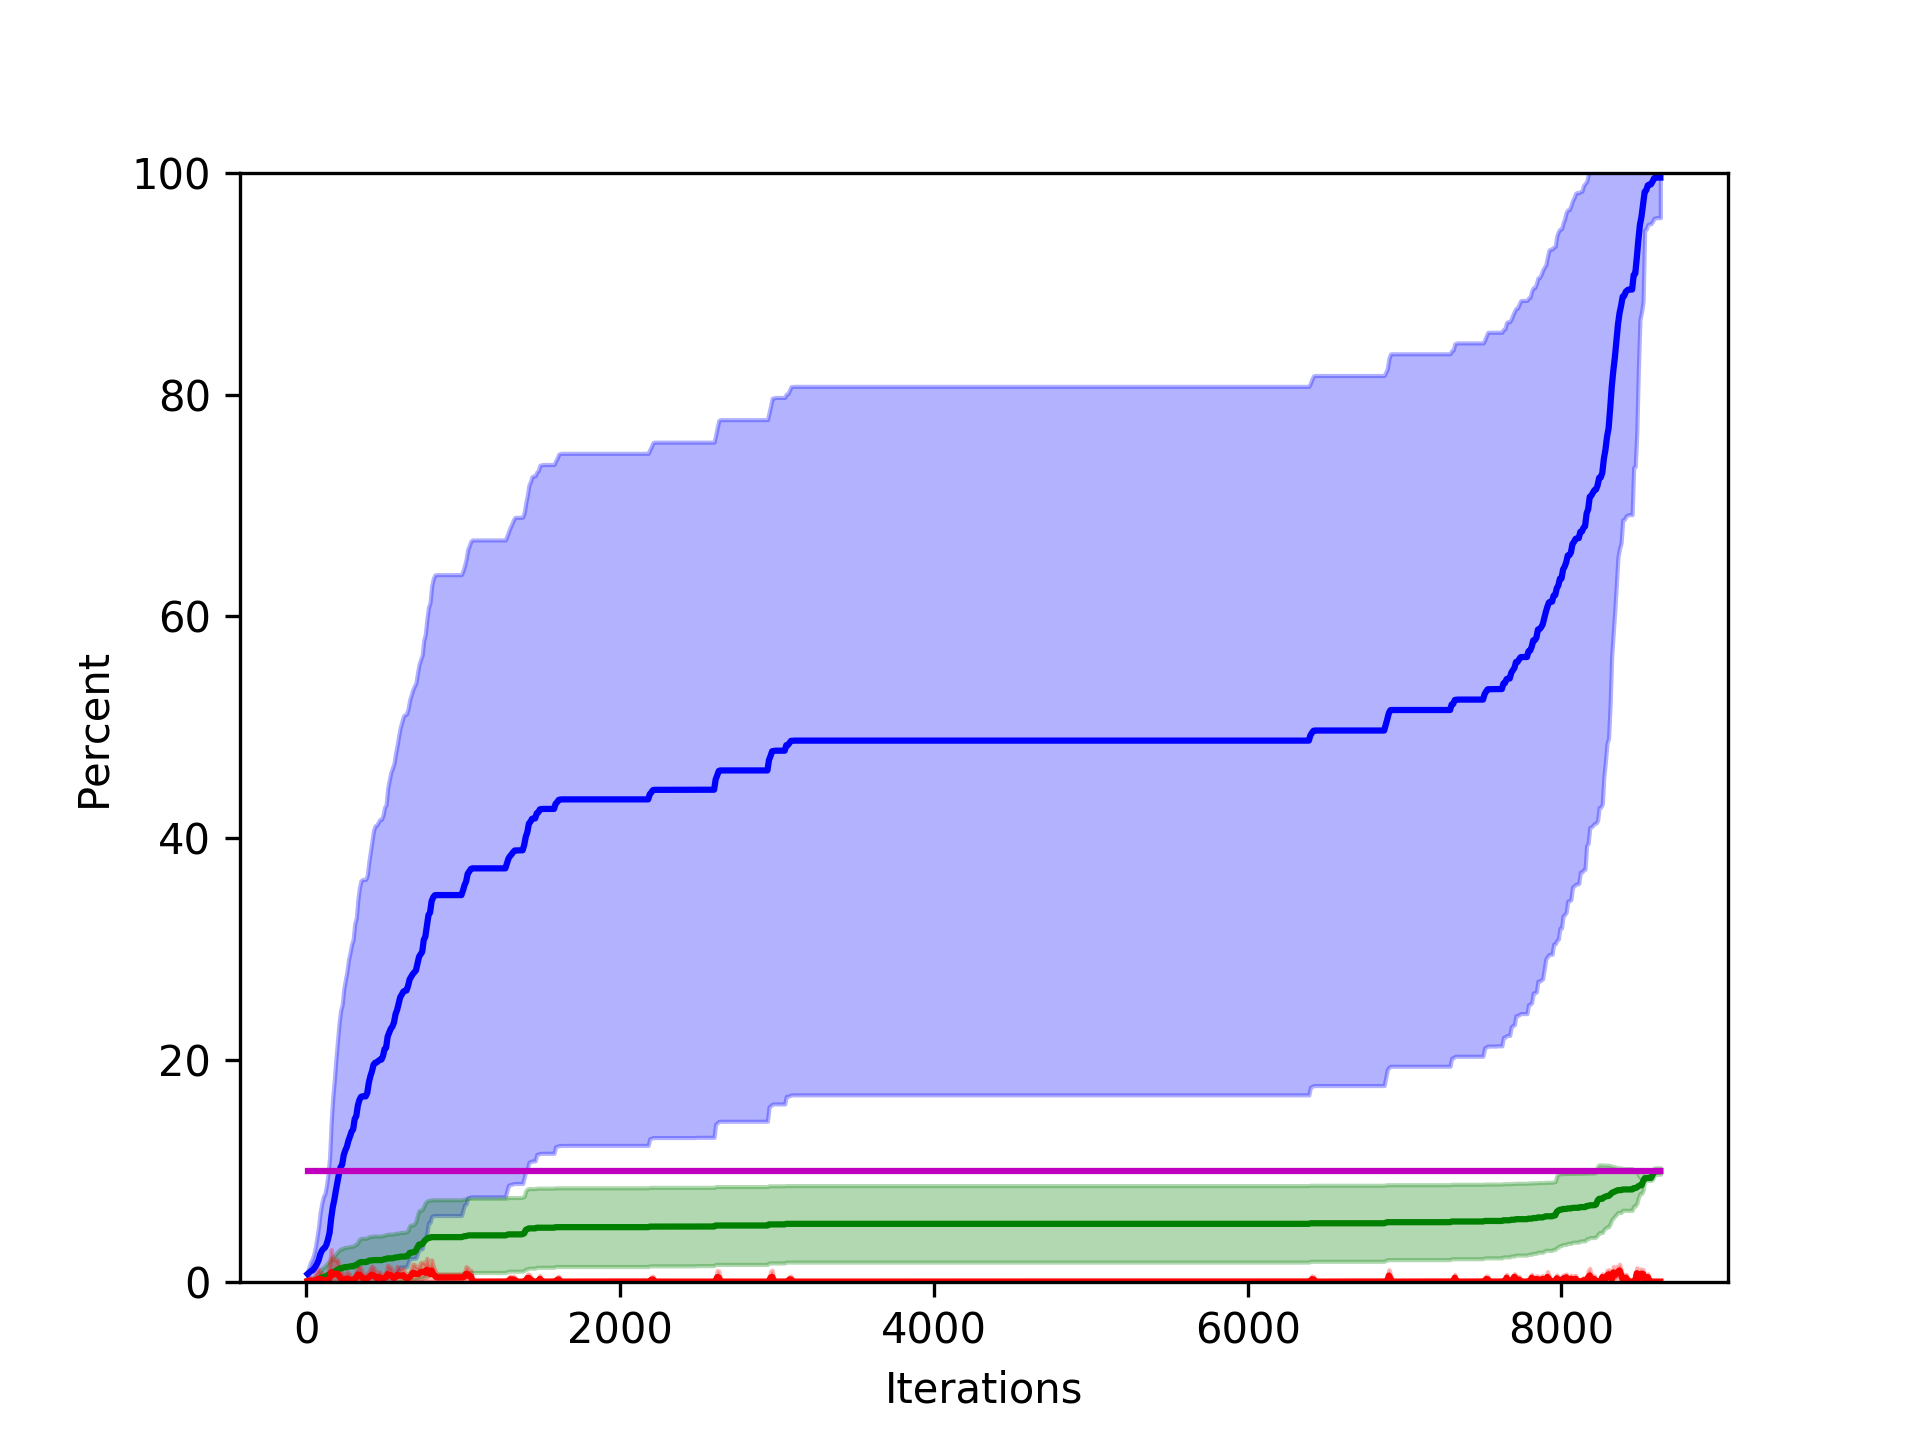
\includegraphics[width=\linewidth]{images/plots/Network_rA_10.0/new_plots/10_10.png}
\caption{$\rho$ = 10m.} \label{fig:tarjan0}
\end{subfigure}

\begin{subfigure}{0.6\textwidth}
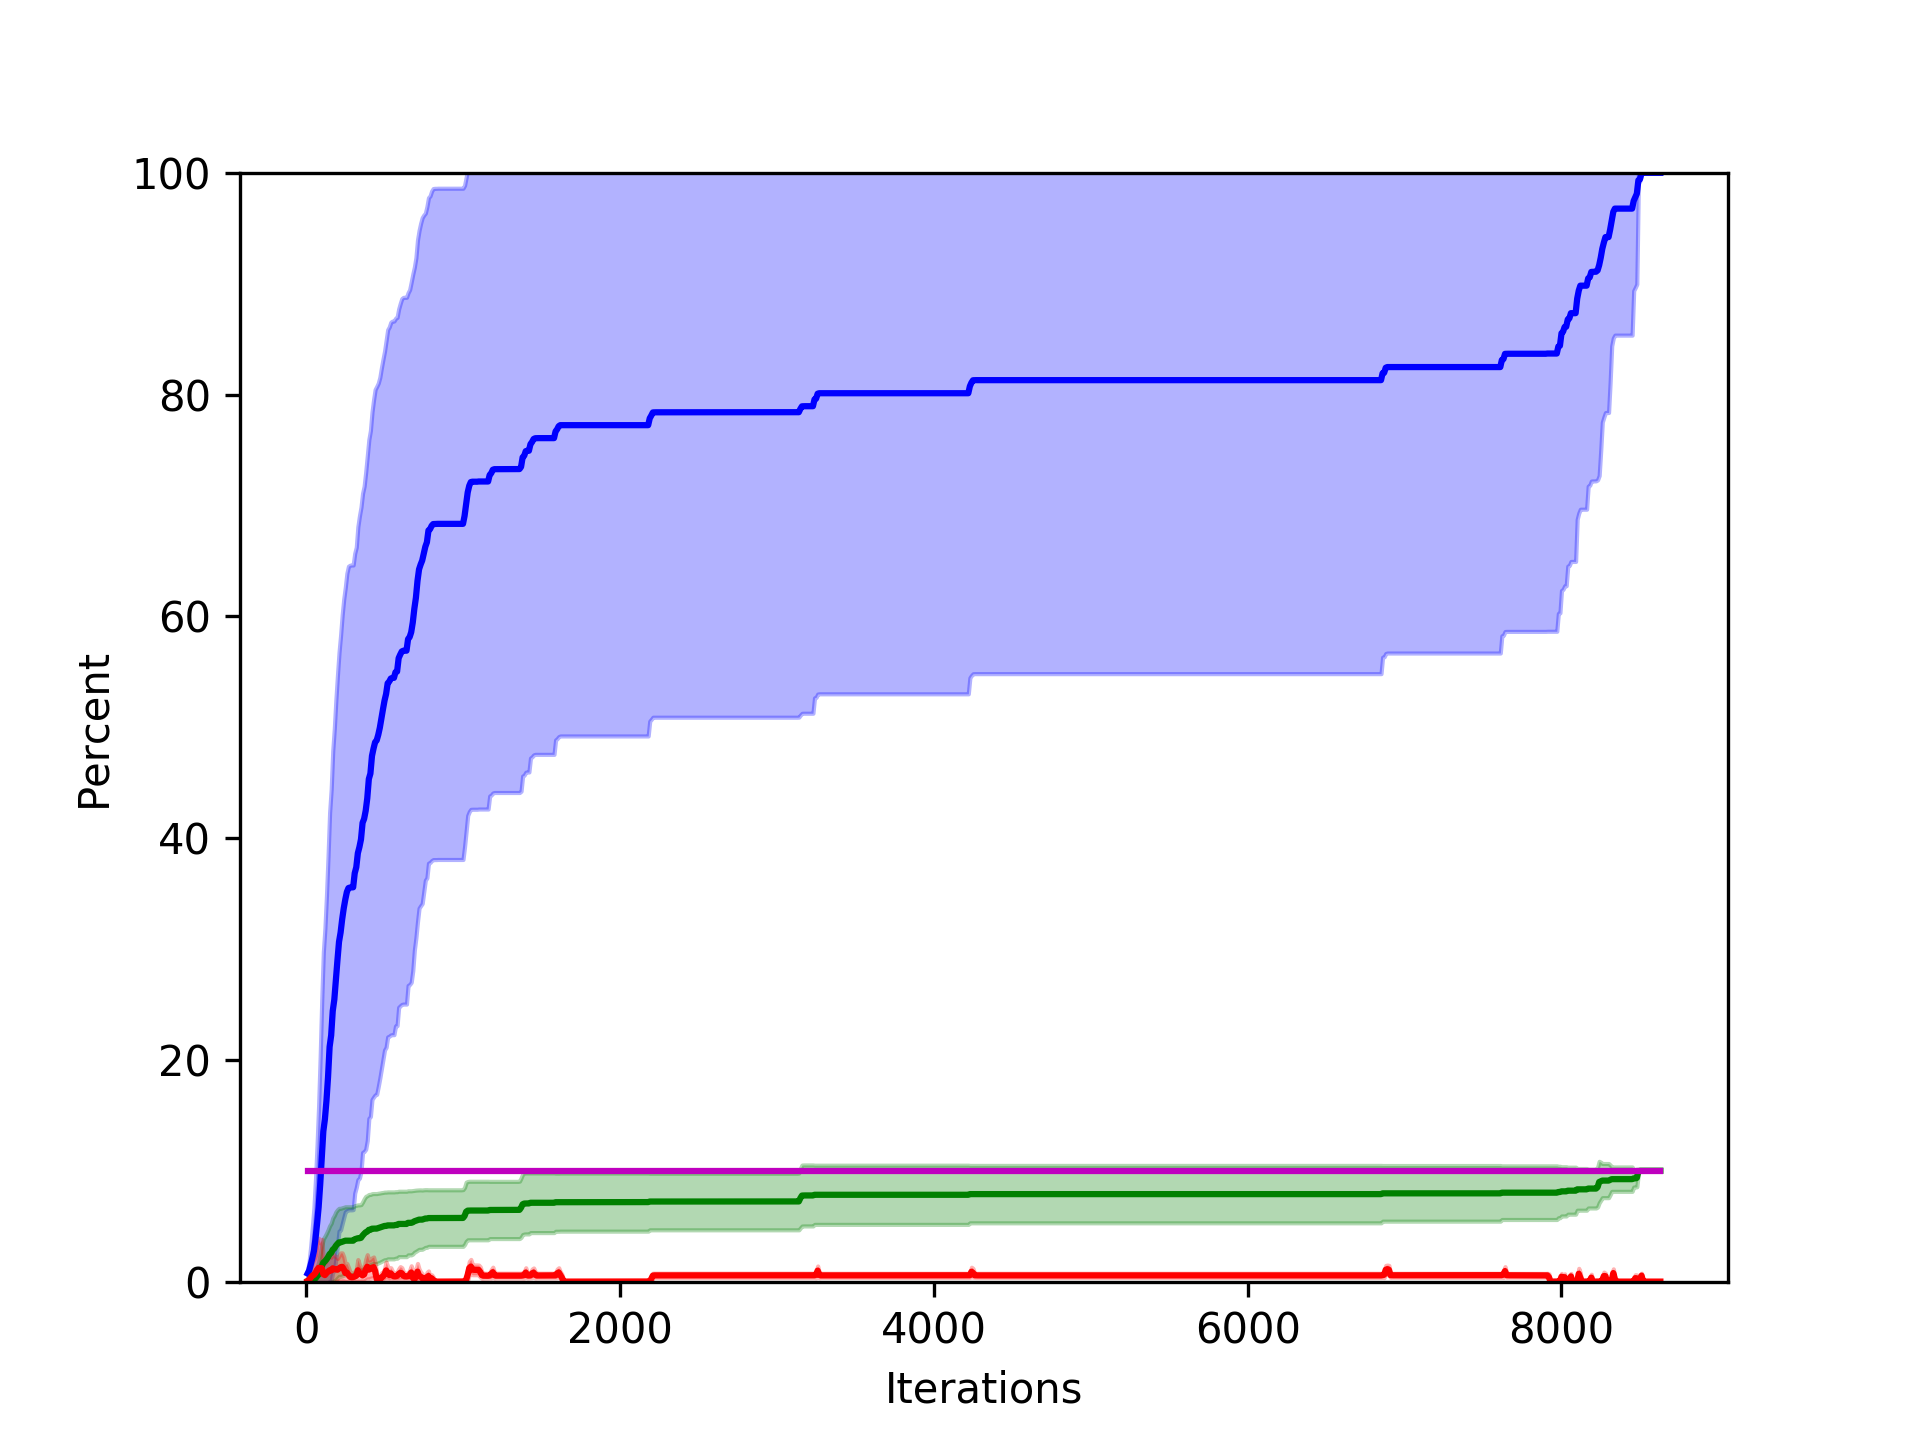
\includegraphics[width=\linewidth]{images/plots/Network_rA_10.0/new_plots/30_10.png}
\caption{$\rho$ = 30m.} \label{fig:tarjan0}
\end{subfigure}

\begin{subfigure}{0.6\textwidth}
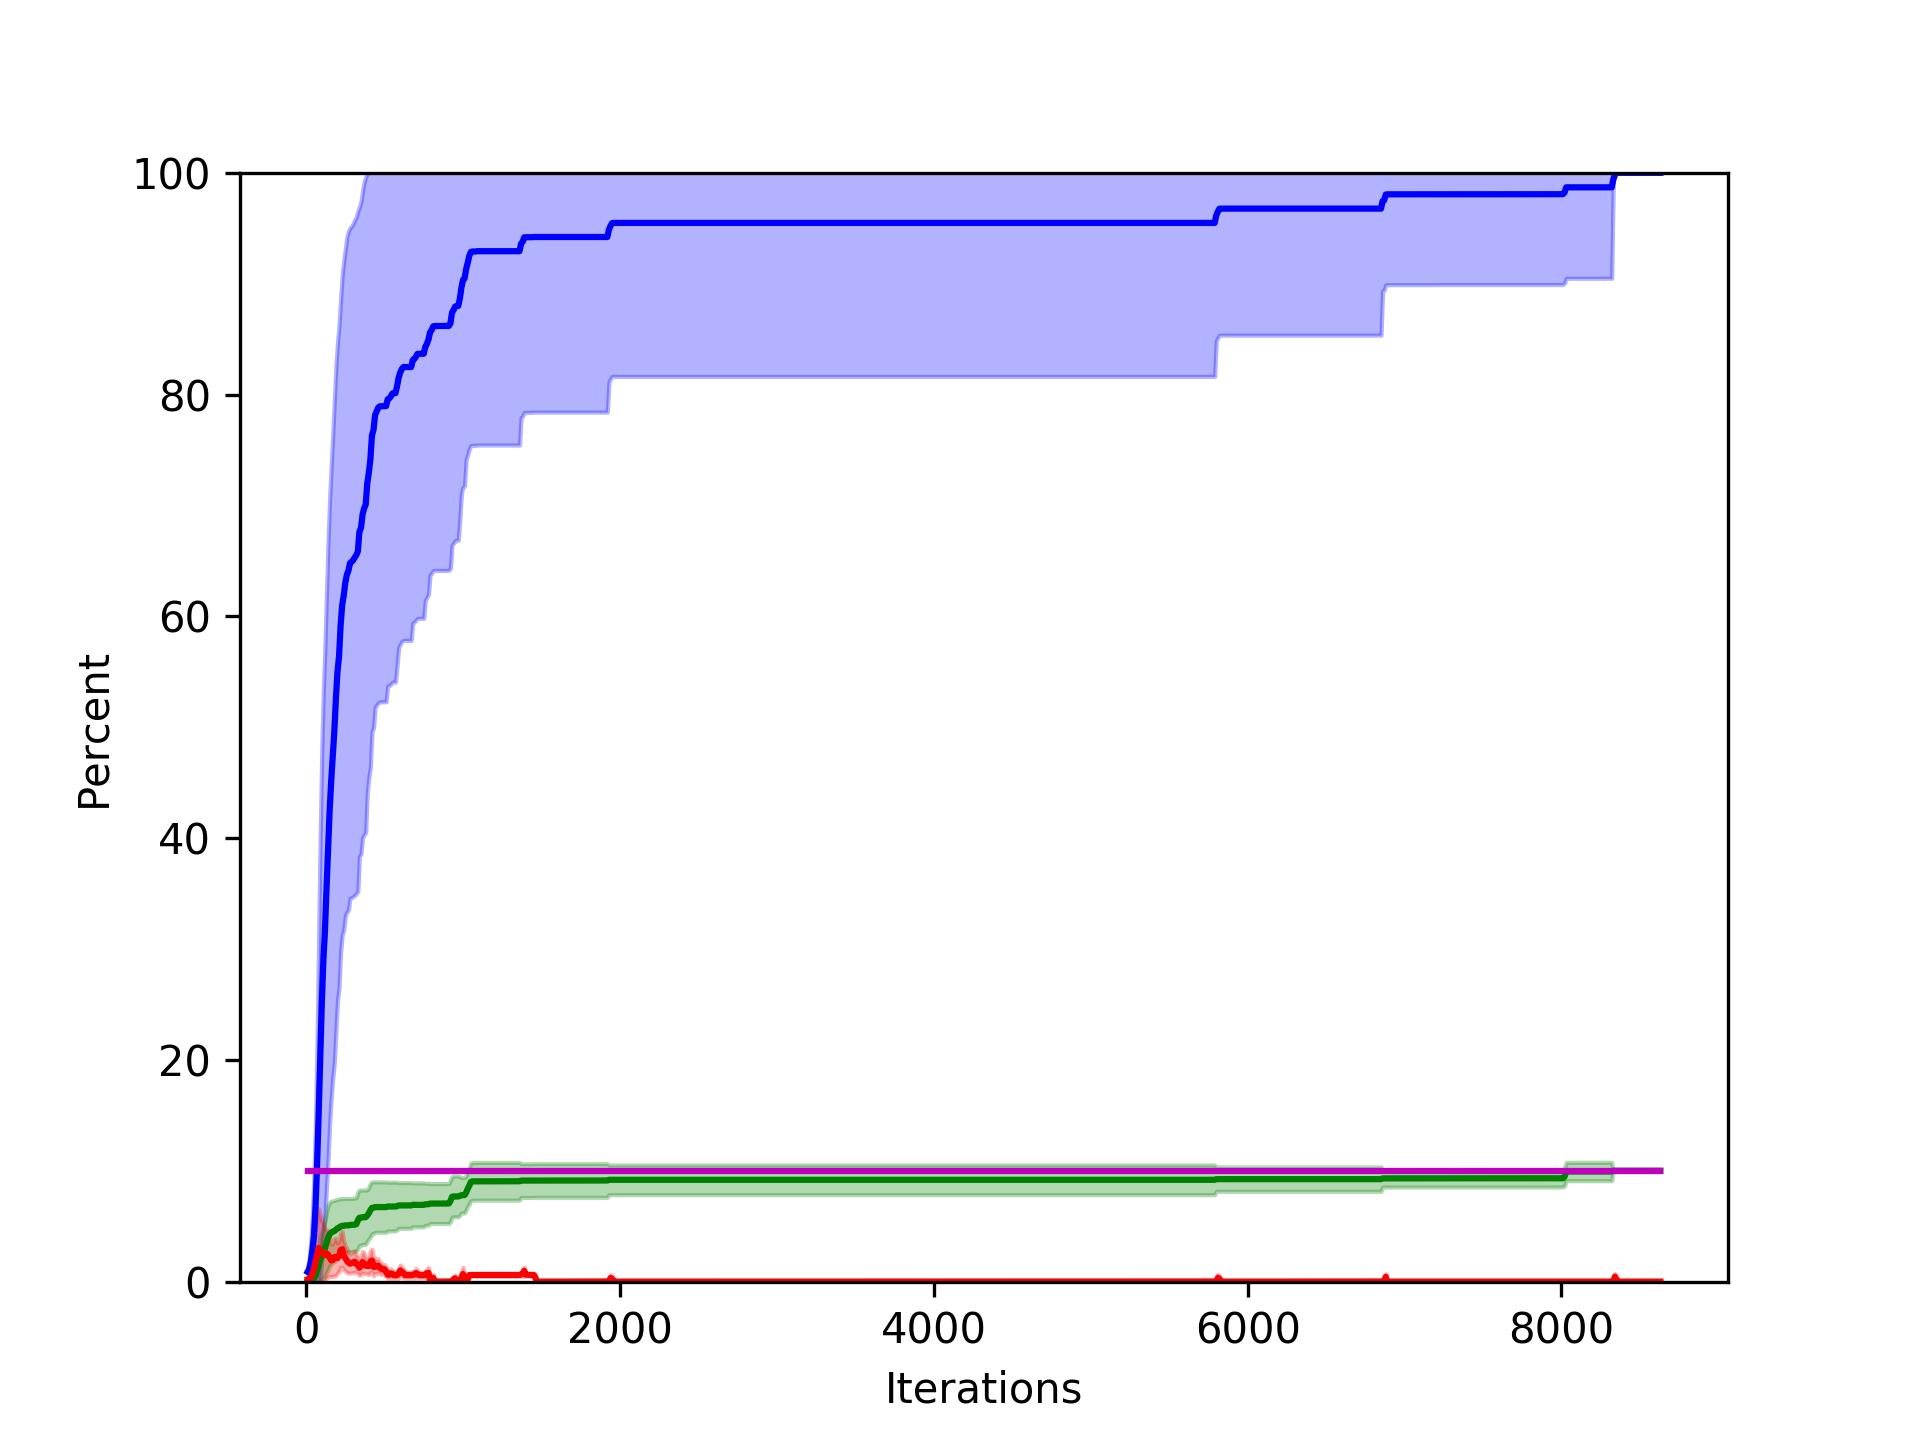
\includegraphics[width=\linewidth]{images/plots/Network_rA_10.0/new_plots/50_10.png}
\caption{$\rho$ = 50m.} \label{fig:tarjan0}
\end{subfigure}

\caption{Simulation with 10\% malicious nodes and varying values of $\rho$.}
\label{fig:random103050}
\end{figure}



\begin{figure}
\centering

\begin{subfigure}{0.6\textwidth}
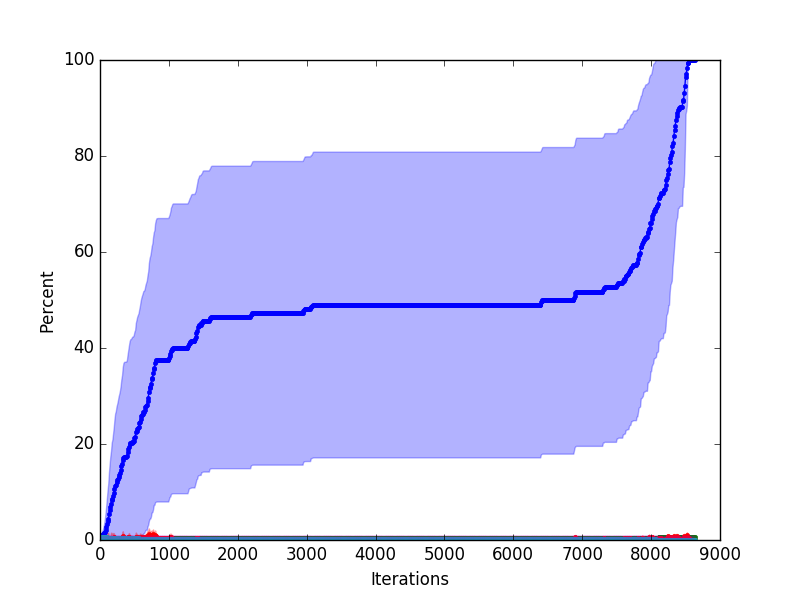
\includegraphics[width=\linewidth]{images/plots/Network_rA/10_1.png}
\caption{1\% malicious.}
\end{subfigure}

\begin{subfigure}{0.6\textwidth}
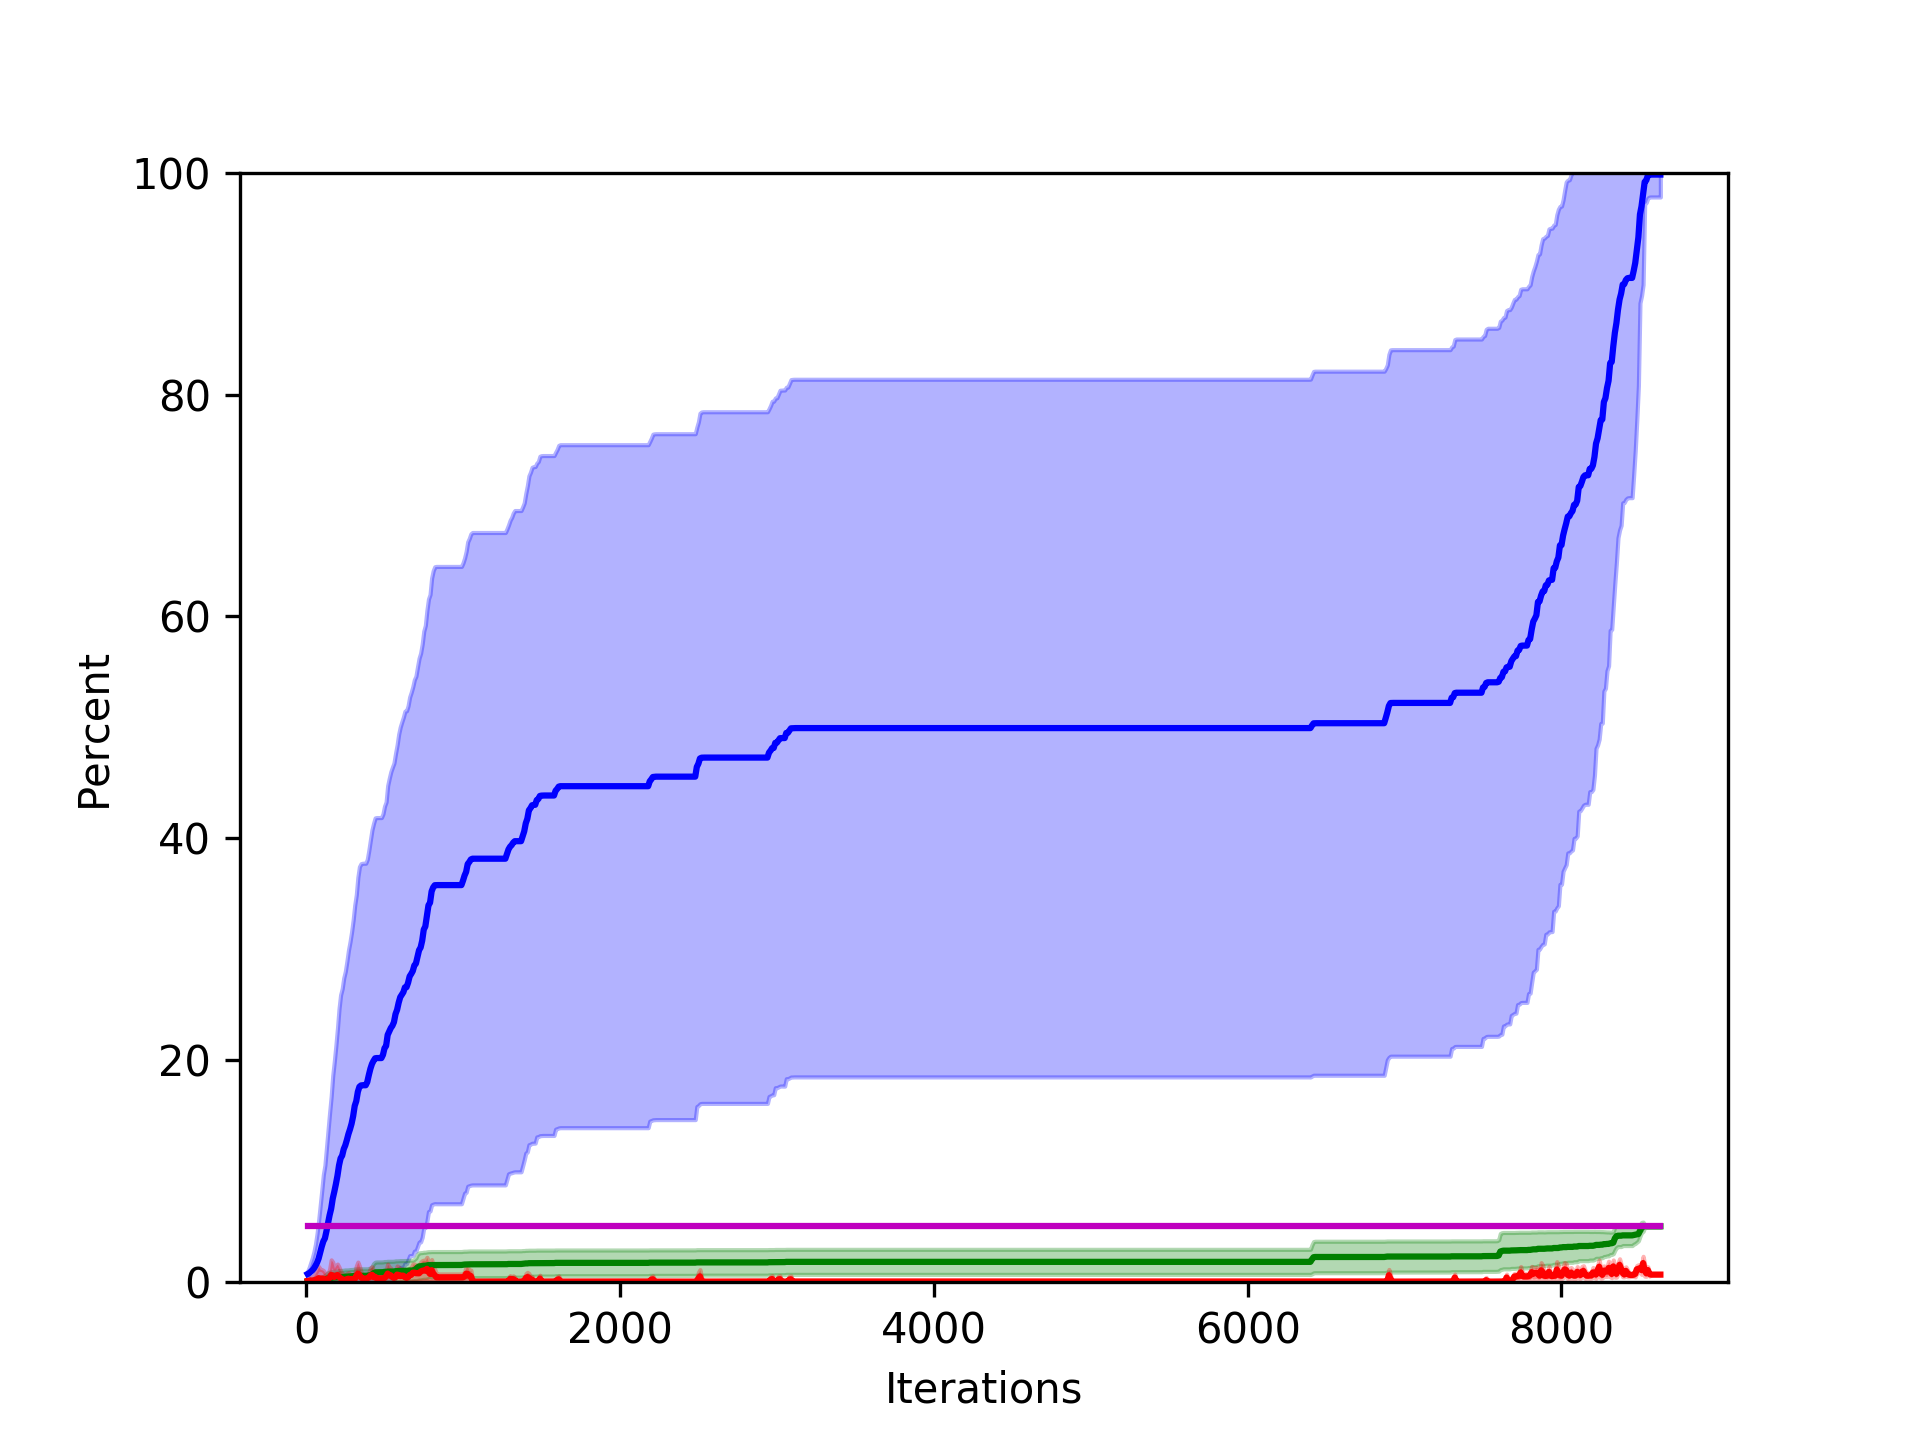
\includegraphics[width=\linewidth]{images/plots/Network_rA/10_5.png}
\caption{5\% malicious.}
\end{subfigure}

\begin{subfigure}{0.6\textwidth}
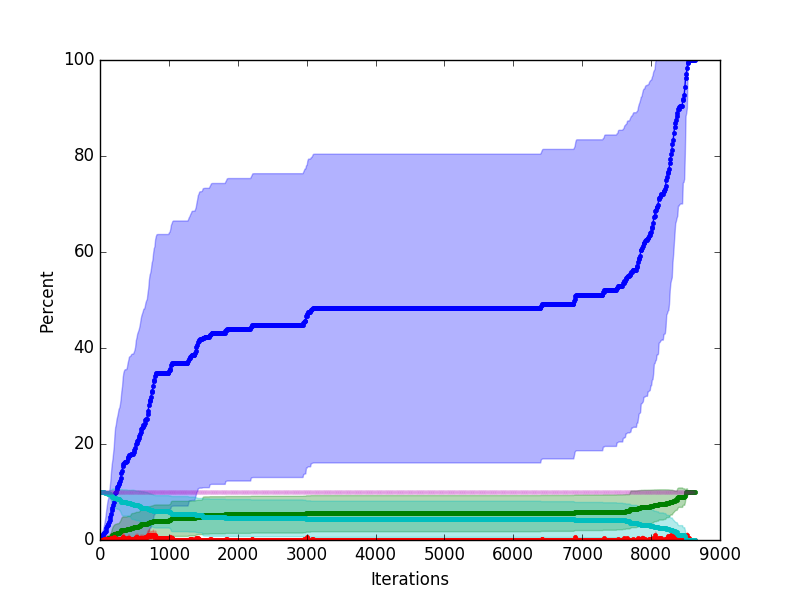
\includegraphics[width=\linewidth]{images/plots/Network_rA/10_10.png}
\caption{10\% malicious.}
\end{subfigure}

\caption{Simulation with $\rho$ = 10m and varying percentages of malicious nodes (1\%, 5\% and 10\%).}
\label{fig:randommalicious1}
\end{figure}

\begin{figure}
\centering

\begin{subfigure}{0.6\textwidth}
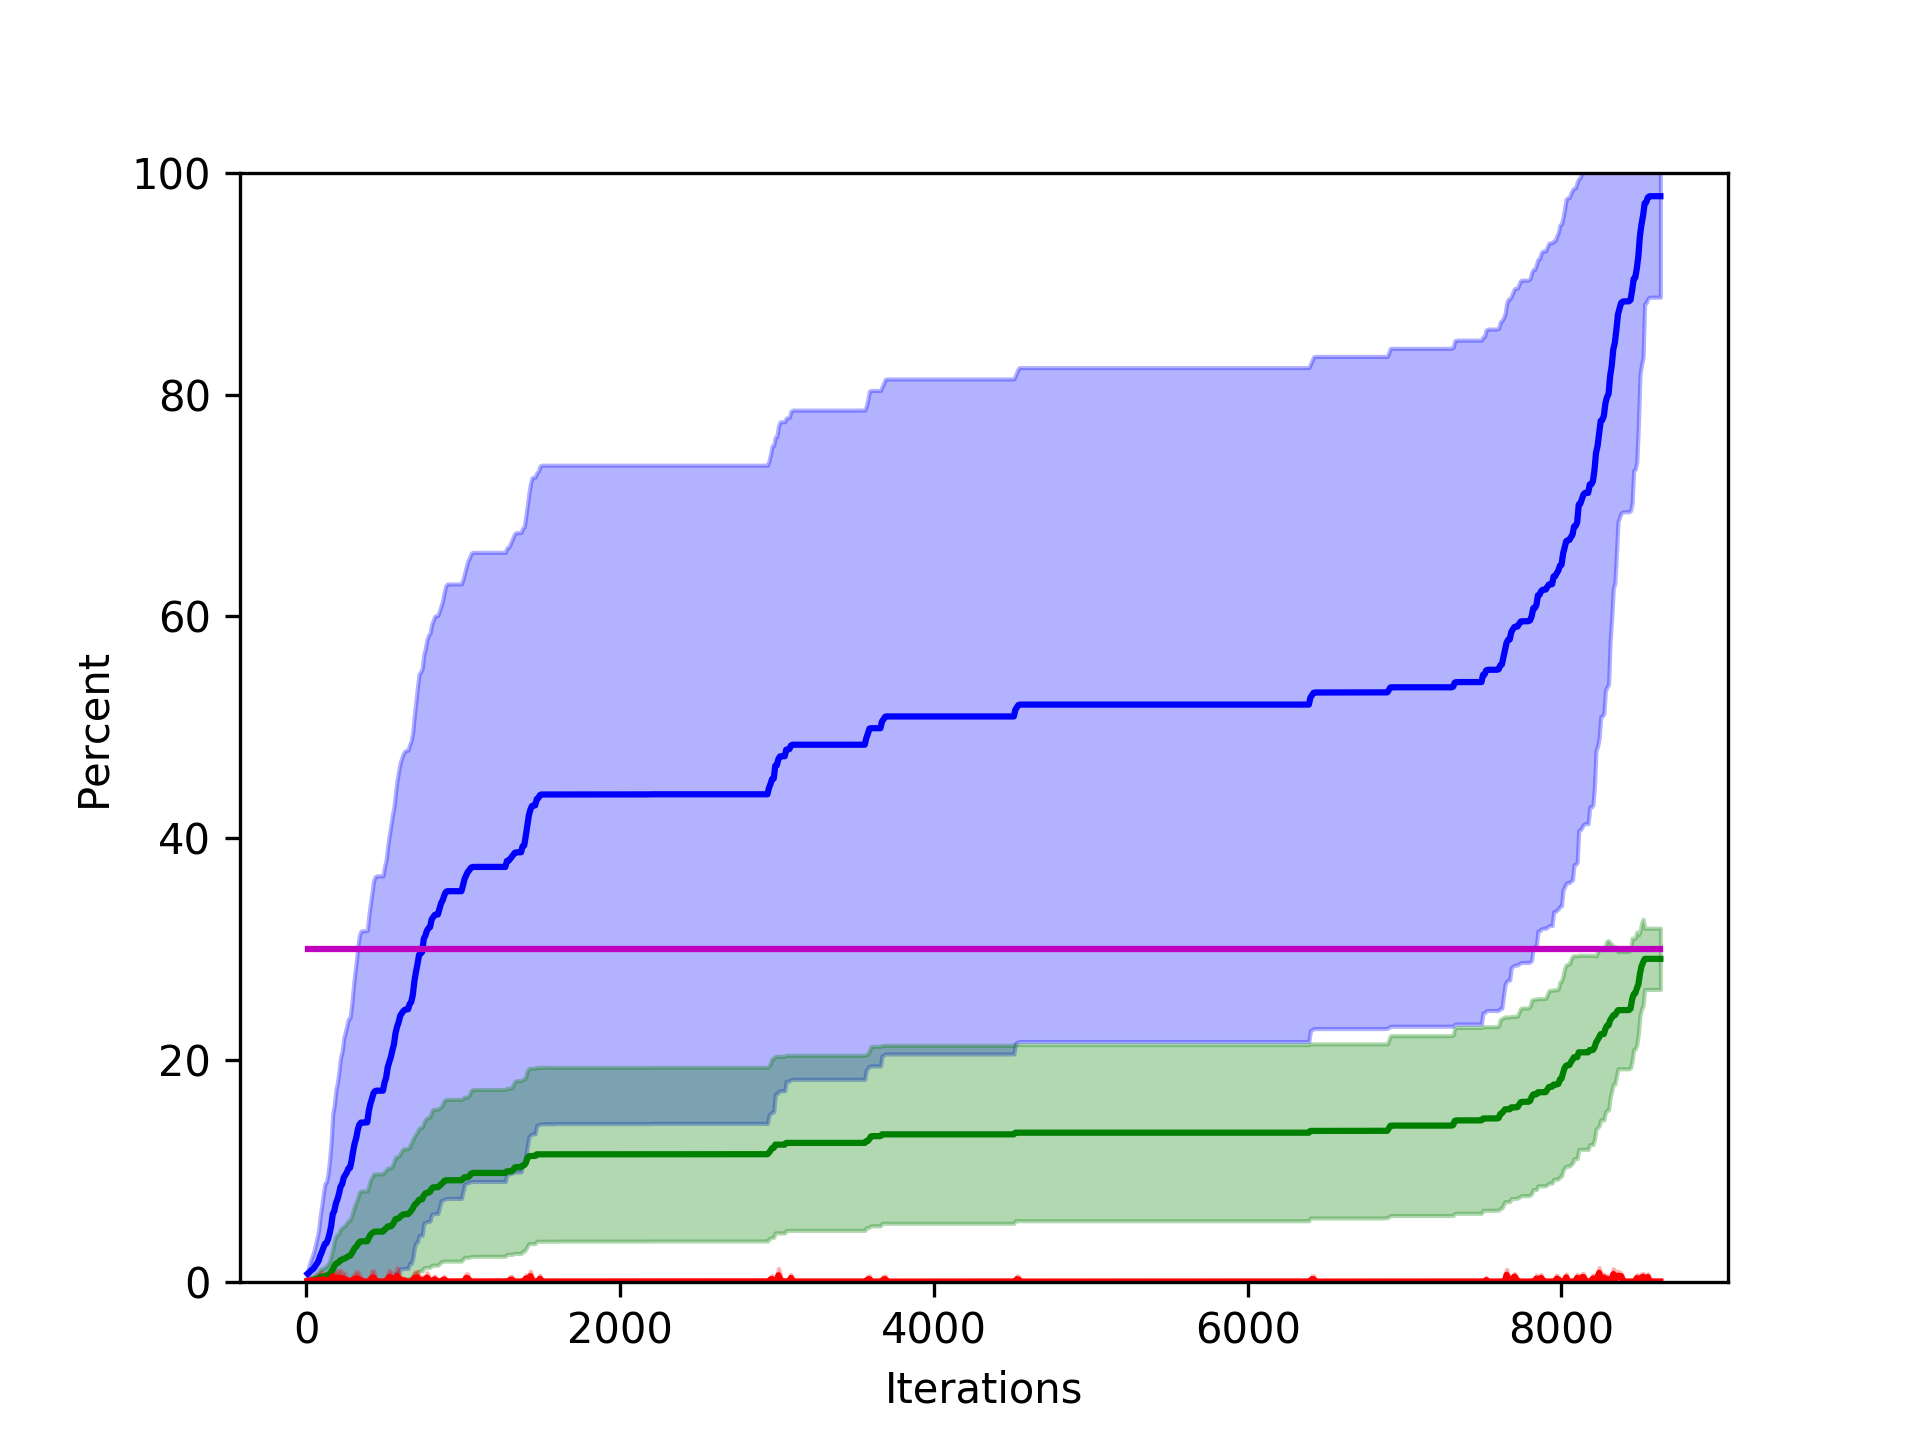
\includegraphics[width=\linewidth]{images/plots/Network_rA/10_30.png}
\caption{30\% malicious.}
\end{subfigure}


\begin{subfigure}{0.6\textwidth}
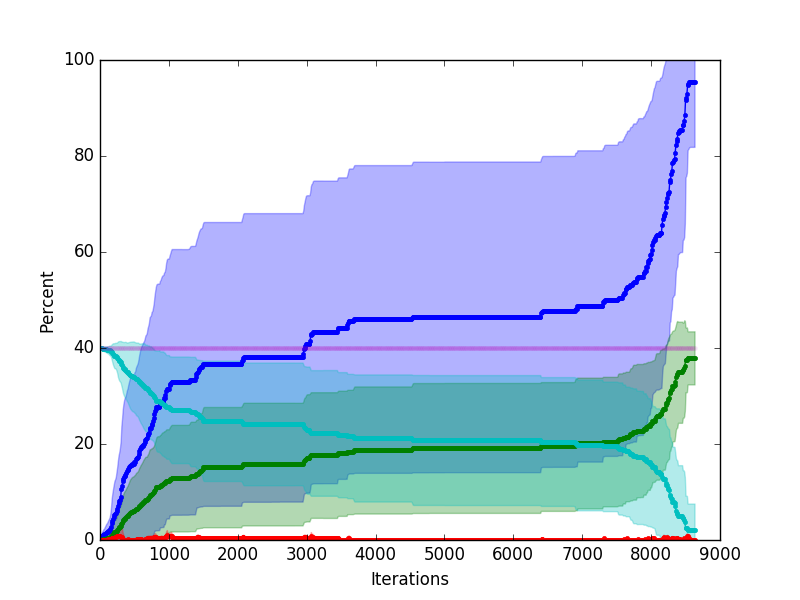
\includegraphics[width=\linewidth]{images/plots/Network_rA/10_40.png}
\caption{40\% malicious.}
\end{subfigure}

\begin{subfigure}{0.6\textwidth}
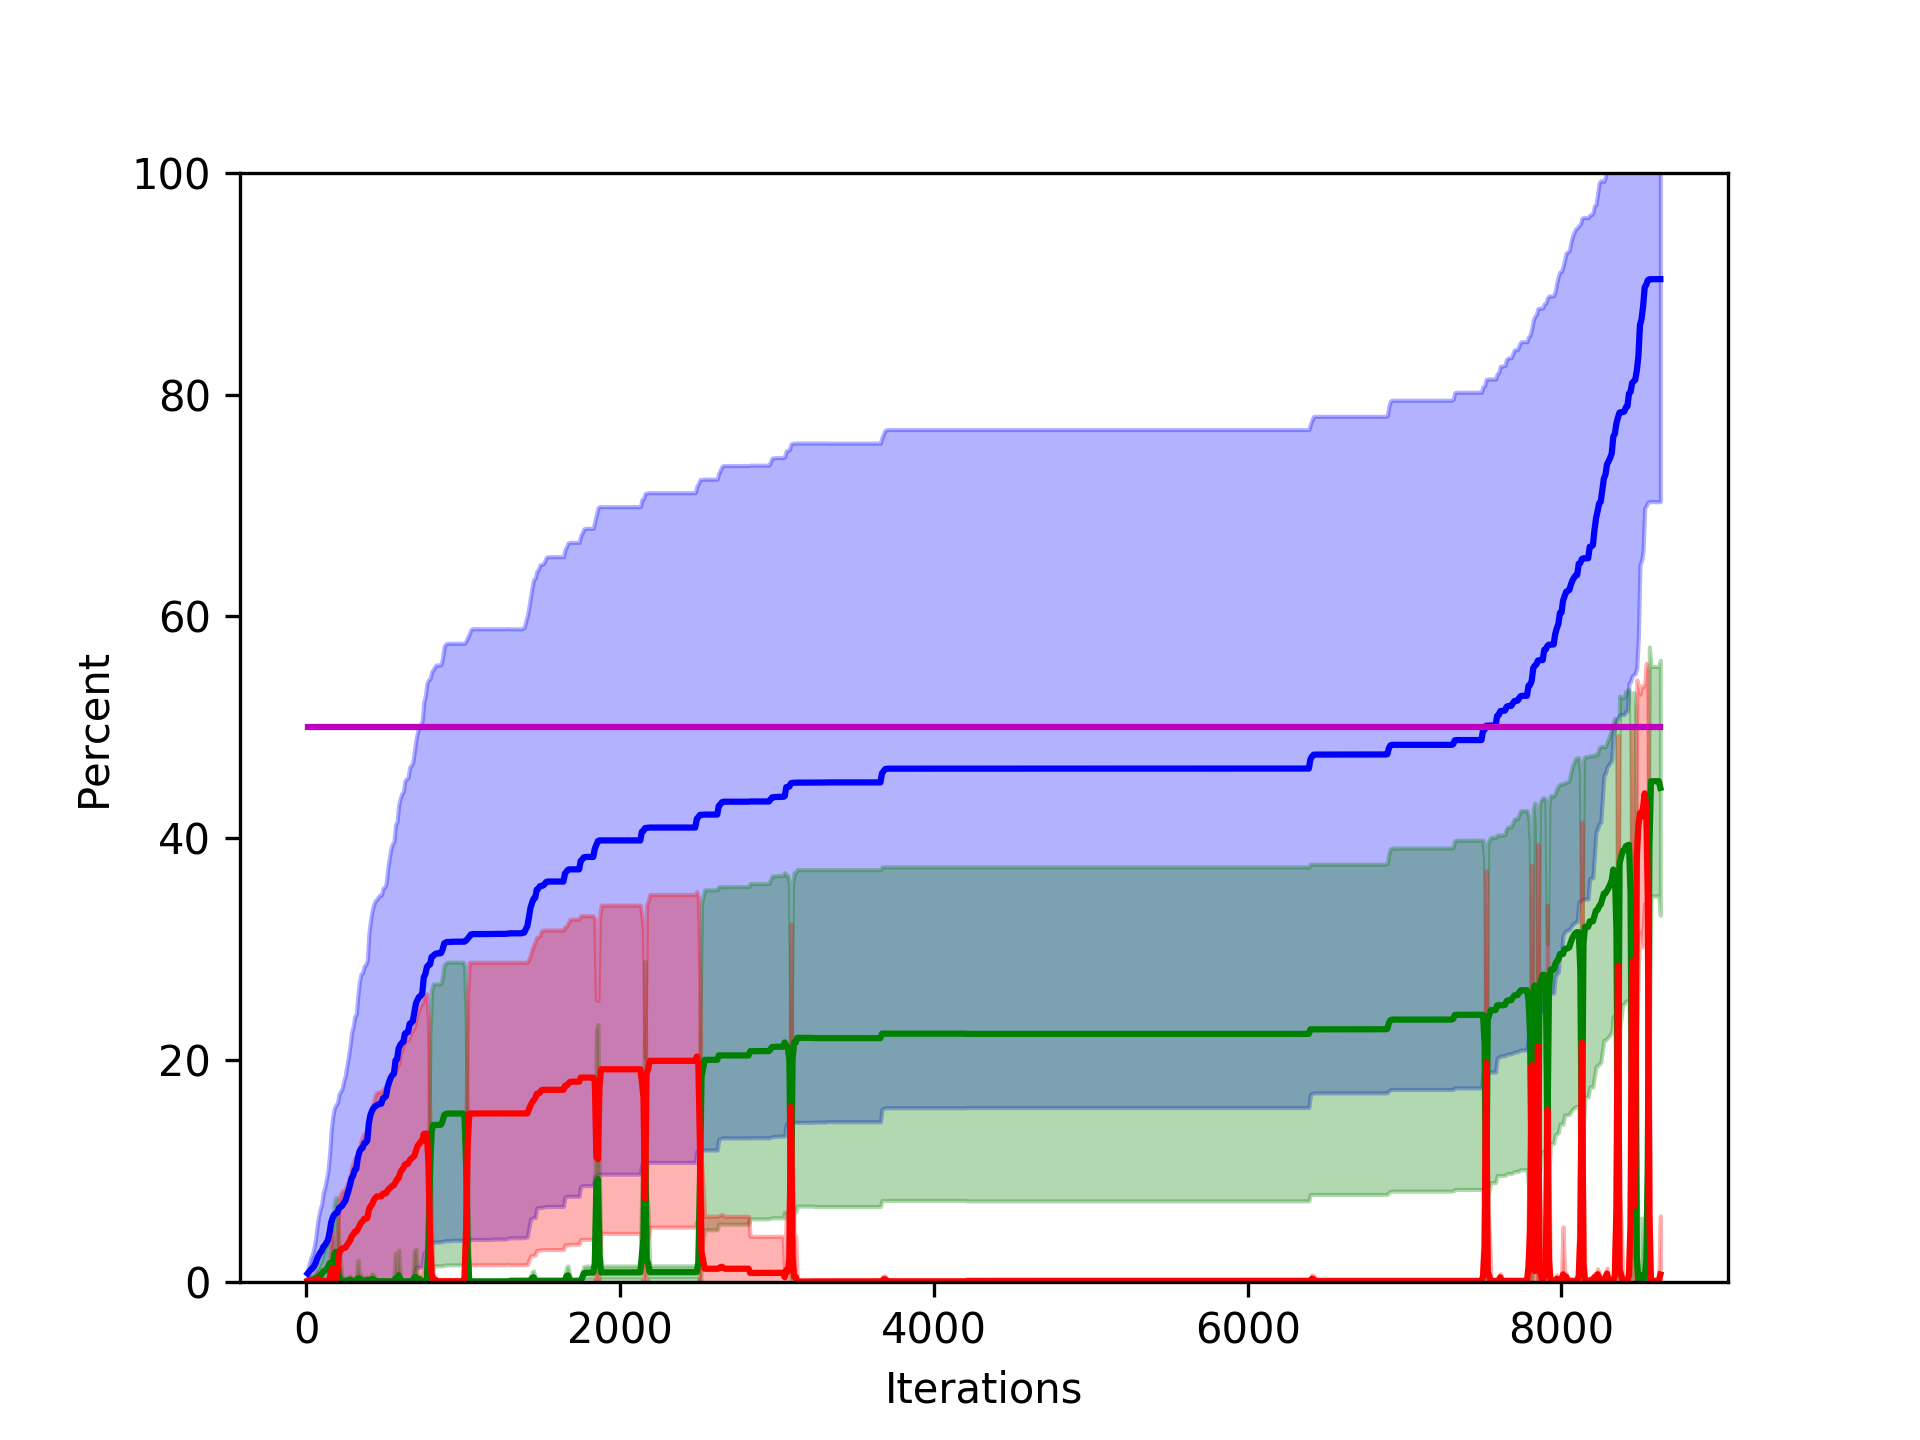
\includegraphics[width=\linewidth]{images/plots/Network_rA/10_50.png}
\caption{50\% malicious.}
\end{subfigure}

\caption{Simulation with $\rho$ = 10m and varying percentages of malicious nodes (30\%, 40\% and 50\%).}
\label{fig:randommalicious2}
\end{figure}


\begin{figure}
\centering

\begin{subfigure}{0.6\textwidth}
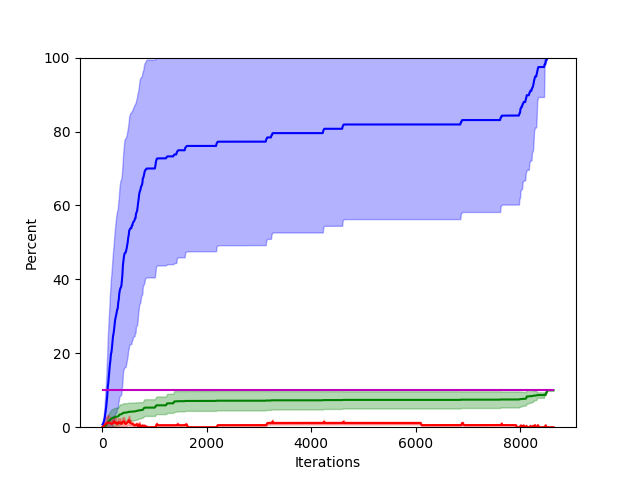
\includegraphics[width=\linewidth]{images/plots/thresholds/03_30_10}
\caption{$h = 0.3$.} \label{fig:threshold03}
\end{subfigure}

\begin{subfigure}{0.6\textwidth}
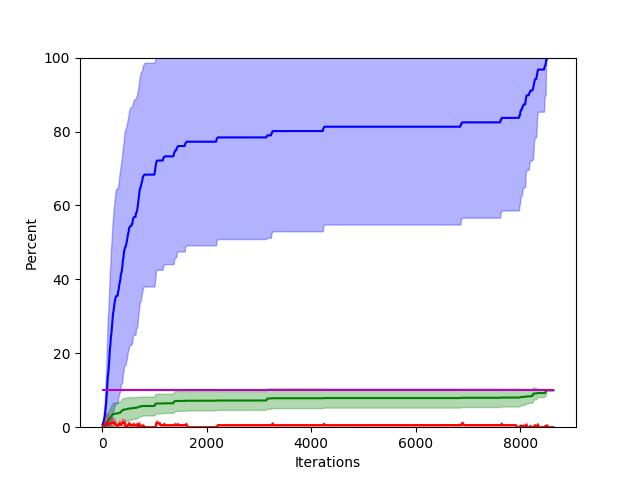
\includegraphics[width=\linewidth]{images/plots/thresholds/05_30_10}
\caption{$h = 0.5$.} \label{fig:threshold05}
\end{subfigure}

\begin{subfigure}{0.6\textwidth}
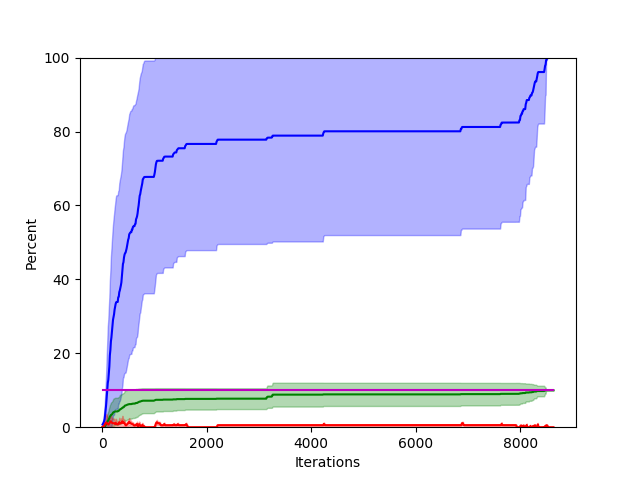
\includegraphics[width=\linewidth]{images/plots/thresholds/07_30_10}
\caption{$h = 0.7$.} \label{fig:threshold07}
\end{subfigure}

\caption{Simulation with 10\% malicious nodes, $\rho = 30$m and varying values of $h$.}
\label{fig:randomthresholds}
\end{figure}


\begin{figure}
\centering
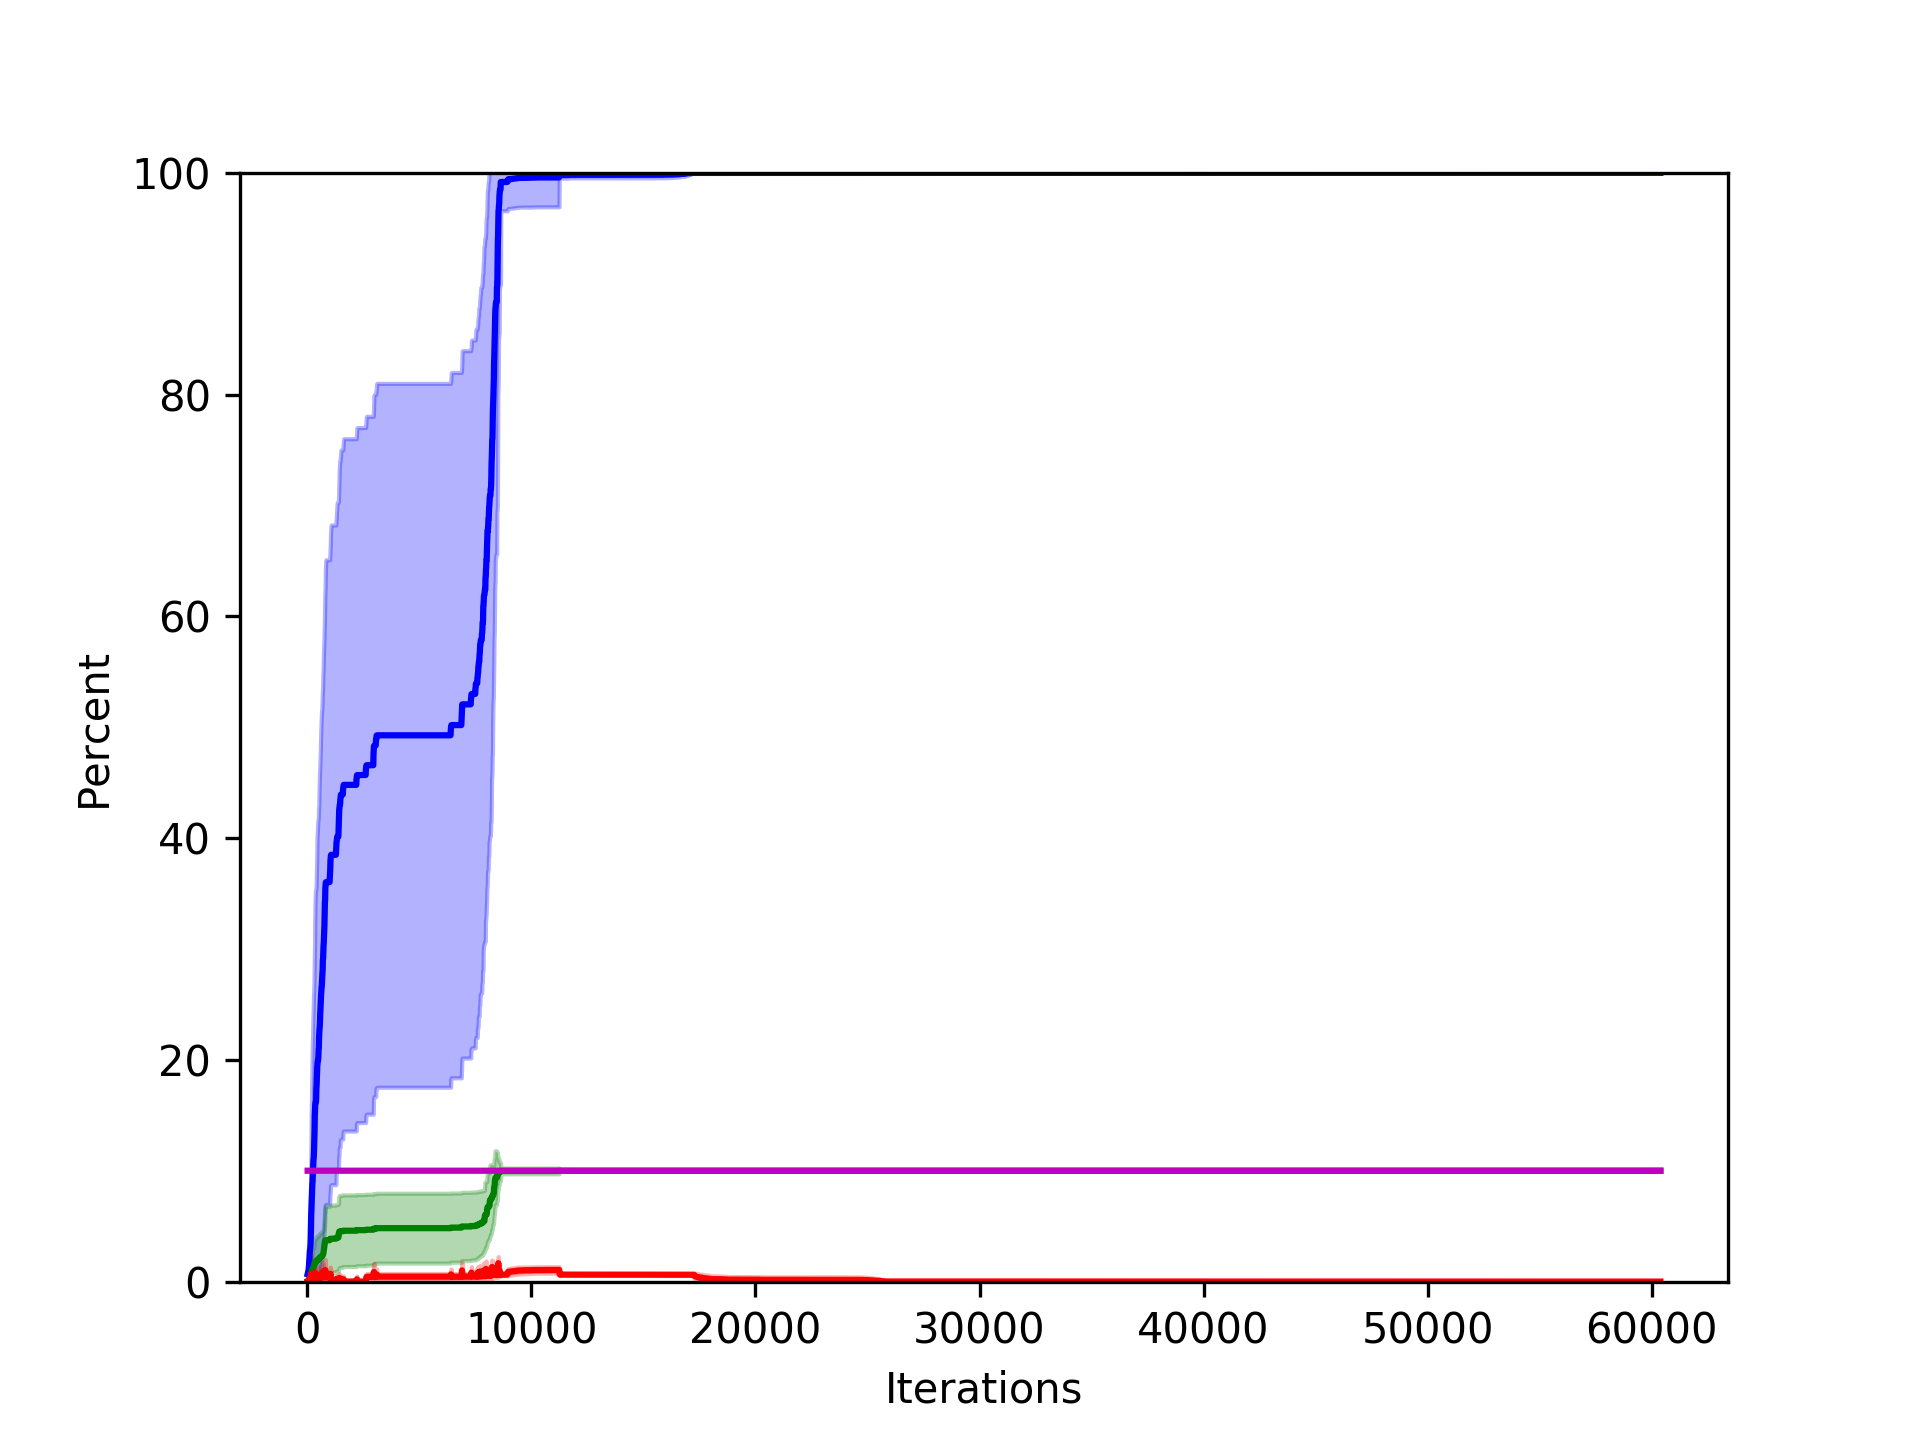
\includegraphics[width=0.6\textwidth]{images/plots/Network_rA7/10_10}
\caption{7 days scenario: 10m range and 10\% malicious nodes.} \label{fig:random7}
\end{figure}


\begin{figure}
\centering

\begin{subfigure}{0.6\textwidth}
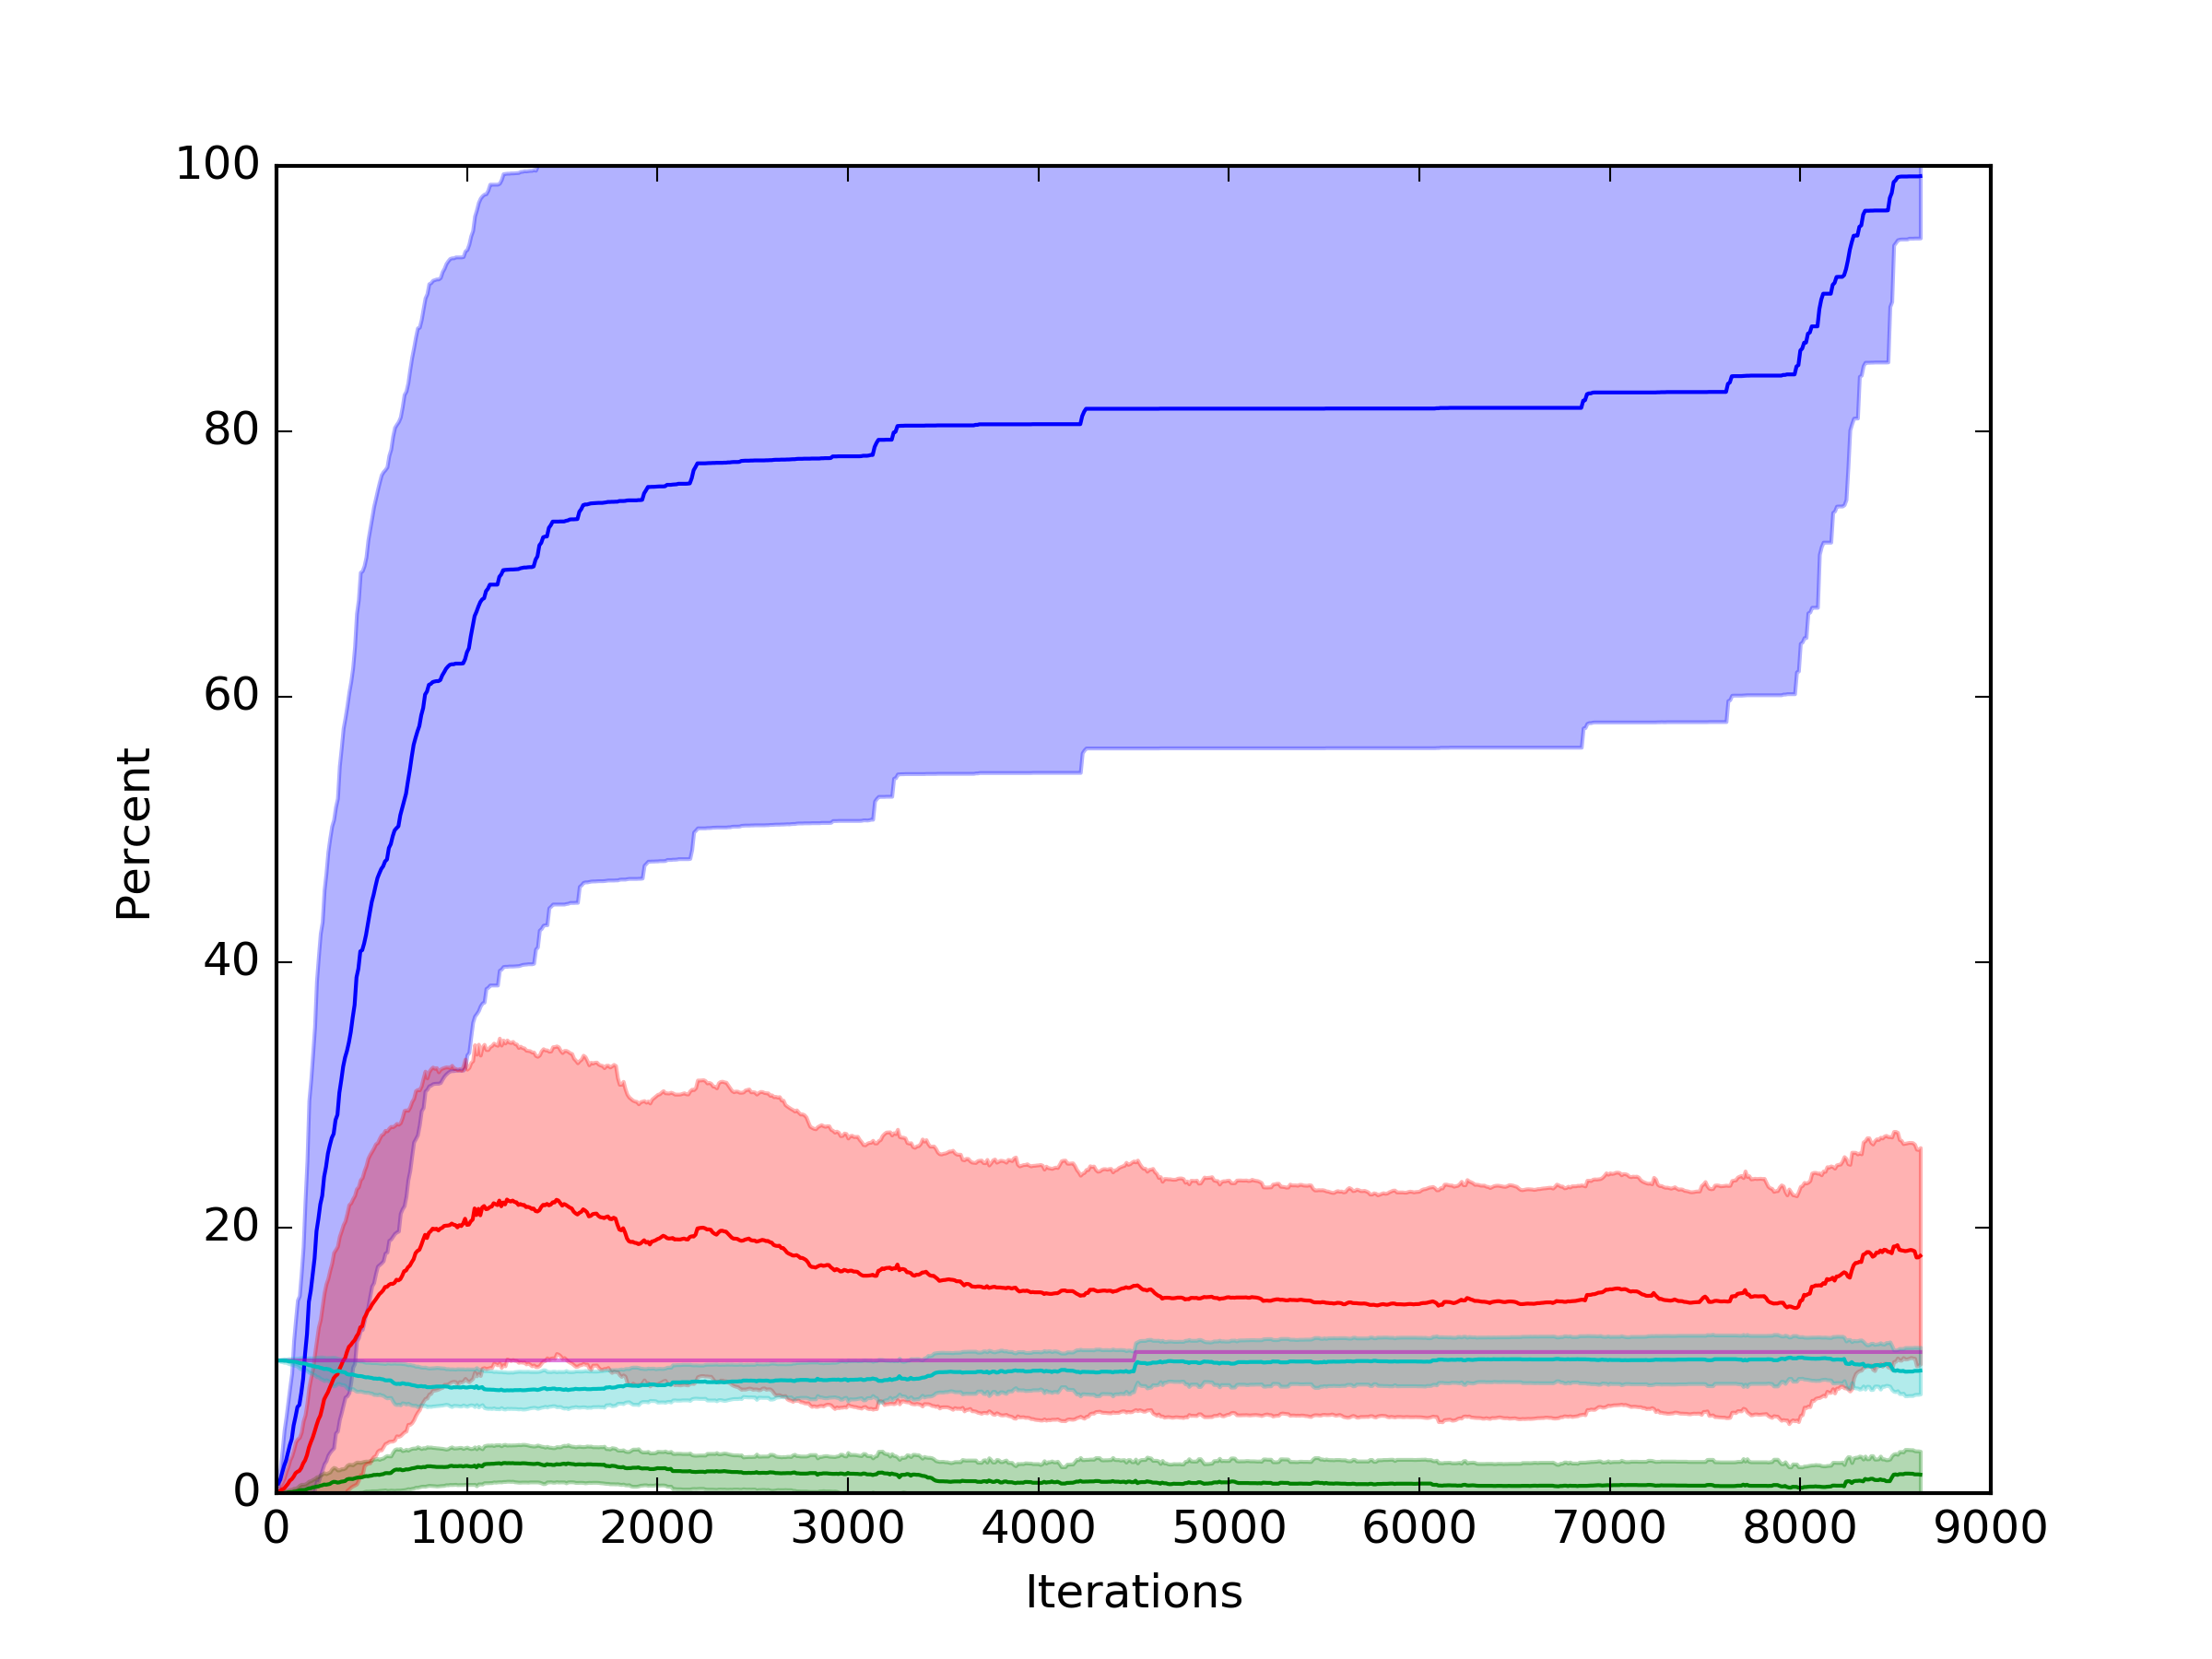
\includegraphics[width=\linewidth]{images/plots/extra_malicious/1_10}
\caption{$m = 10$.} \label{fig:extra10}
\end{subfigure}

\begin{subfigure}{0.6\textwidth}
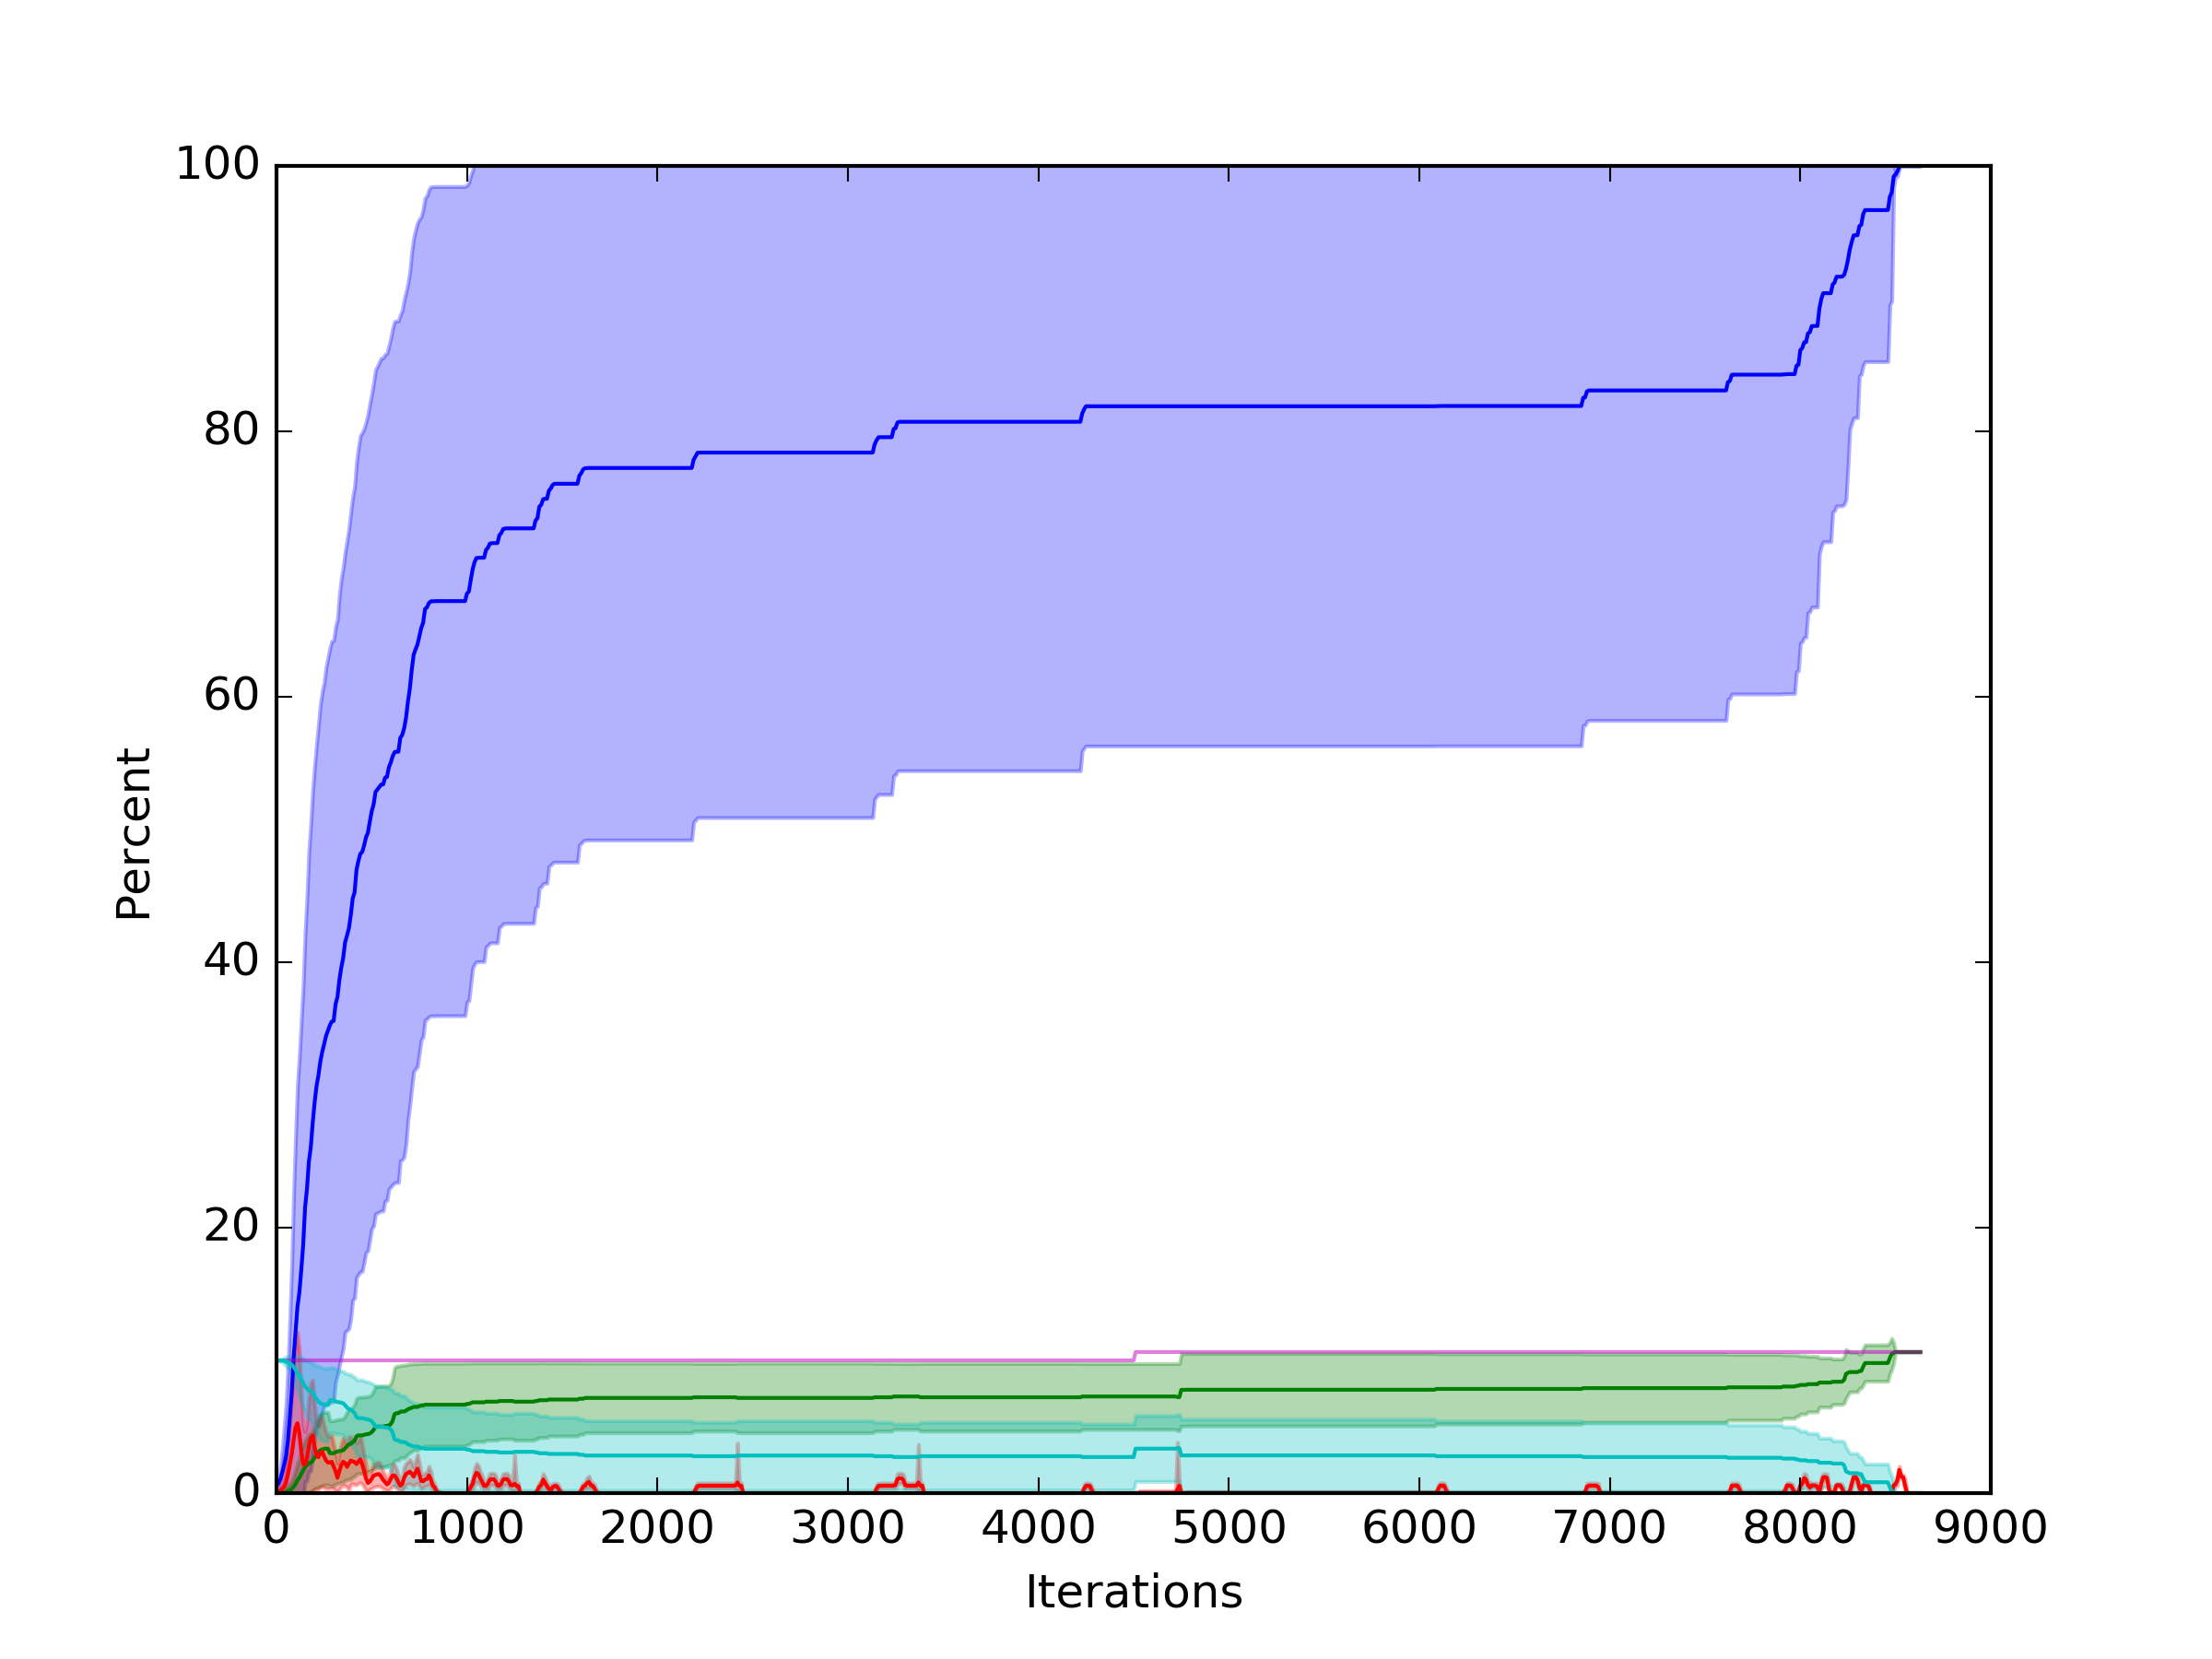
\includegraphics[width=\linewidth]{images/plots/extra_malicious/1_250}
\caption{$m = 250$.} \label{fig:extra250}
\end{subfigure}

\caption{Simulation with information aging, with different maximum age values ($m=10, 250$).}
\label{fig:extramaliciousaging1}
\end{figure}

\begin{figure}
\centering

\begin{subfigure}{0.6\textwidth}
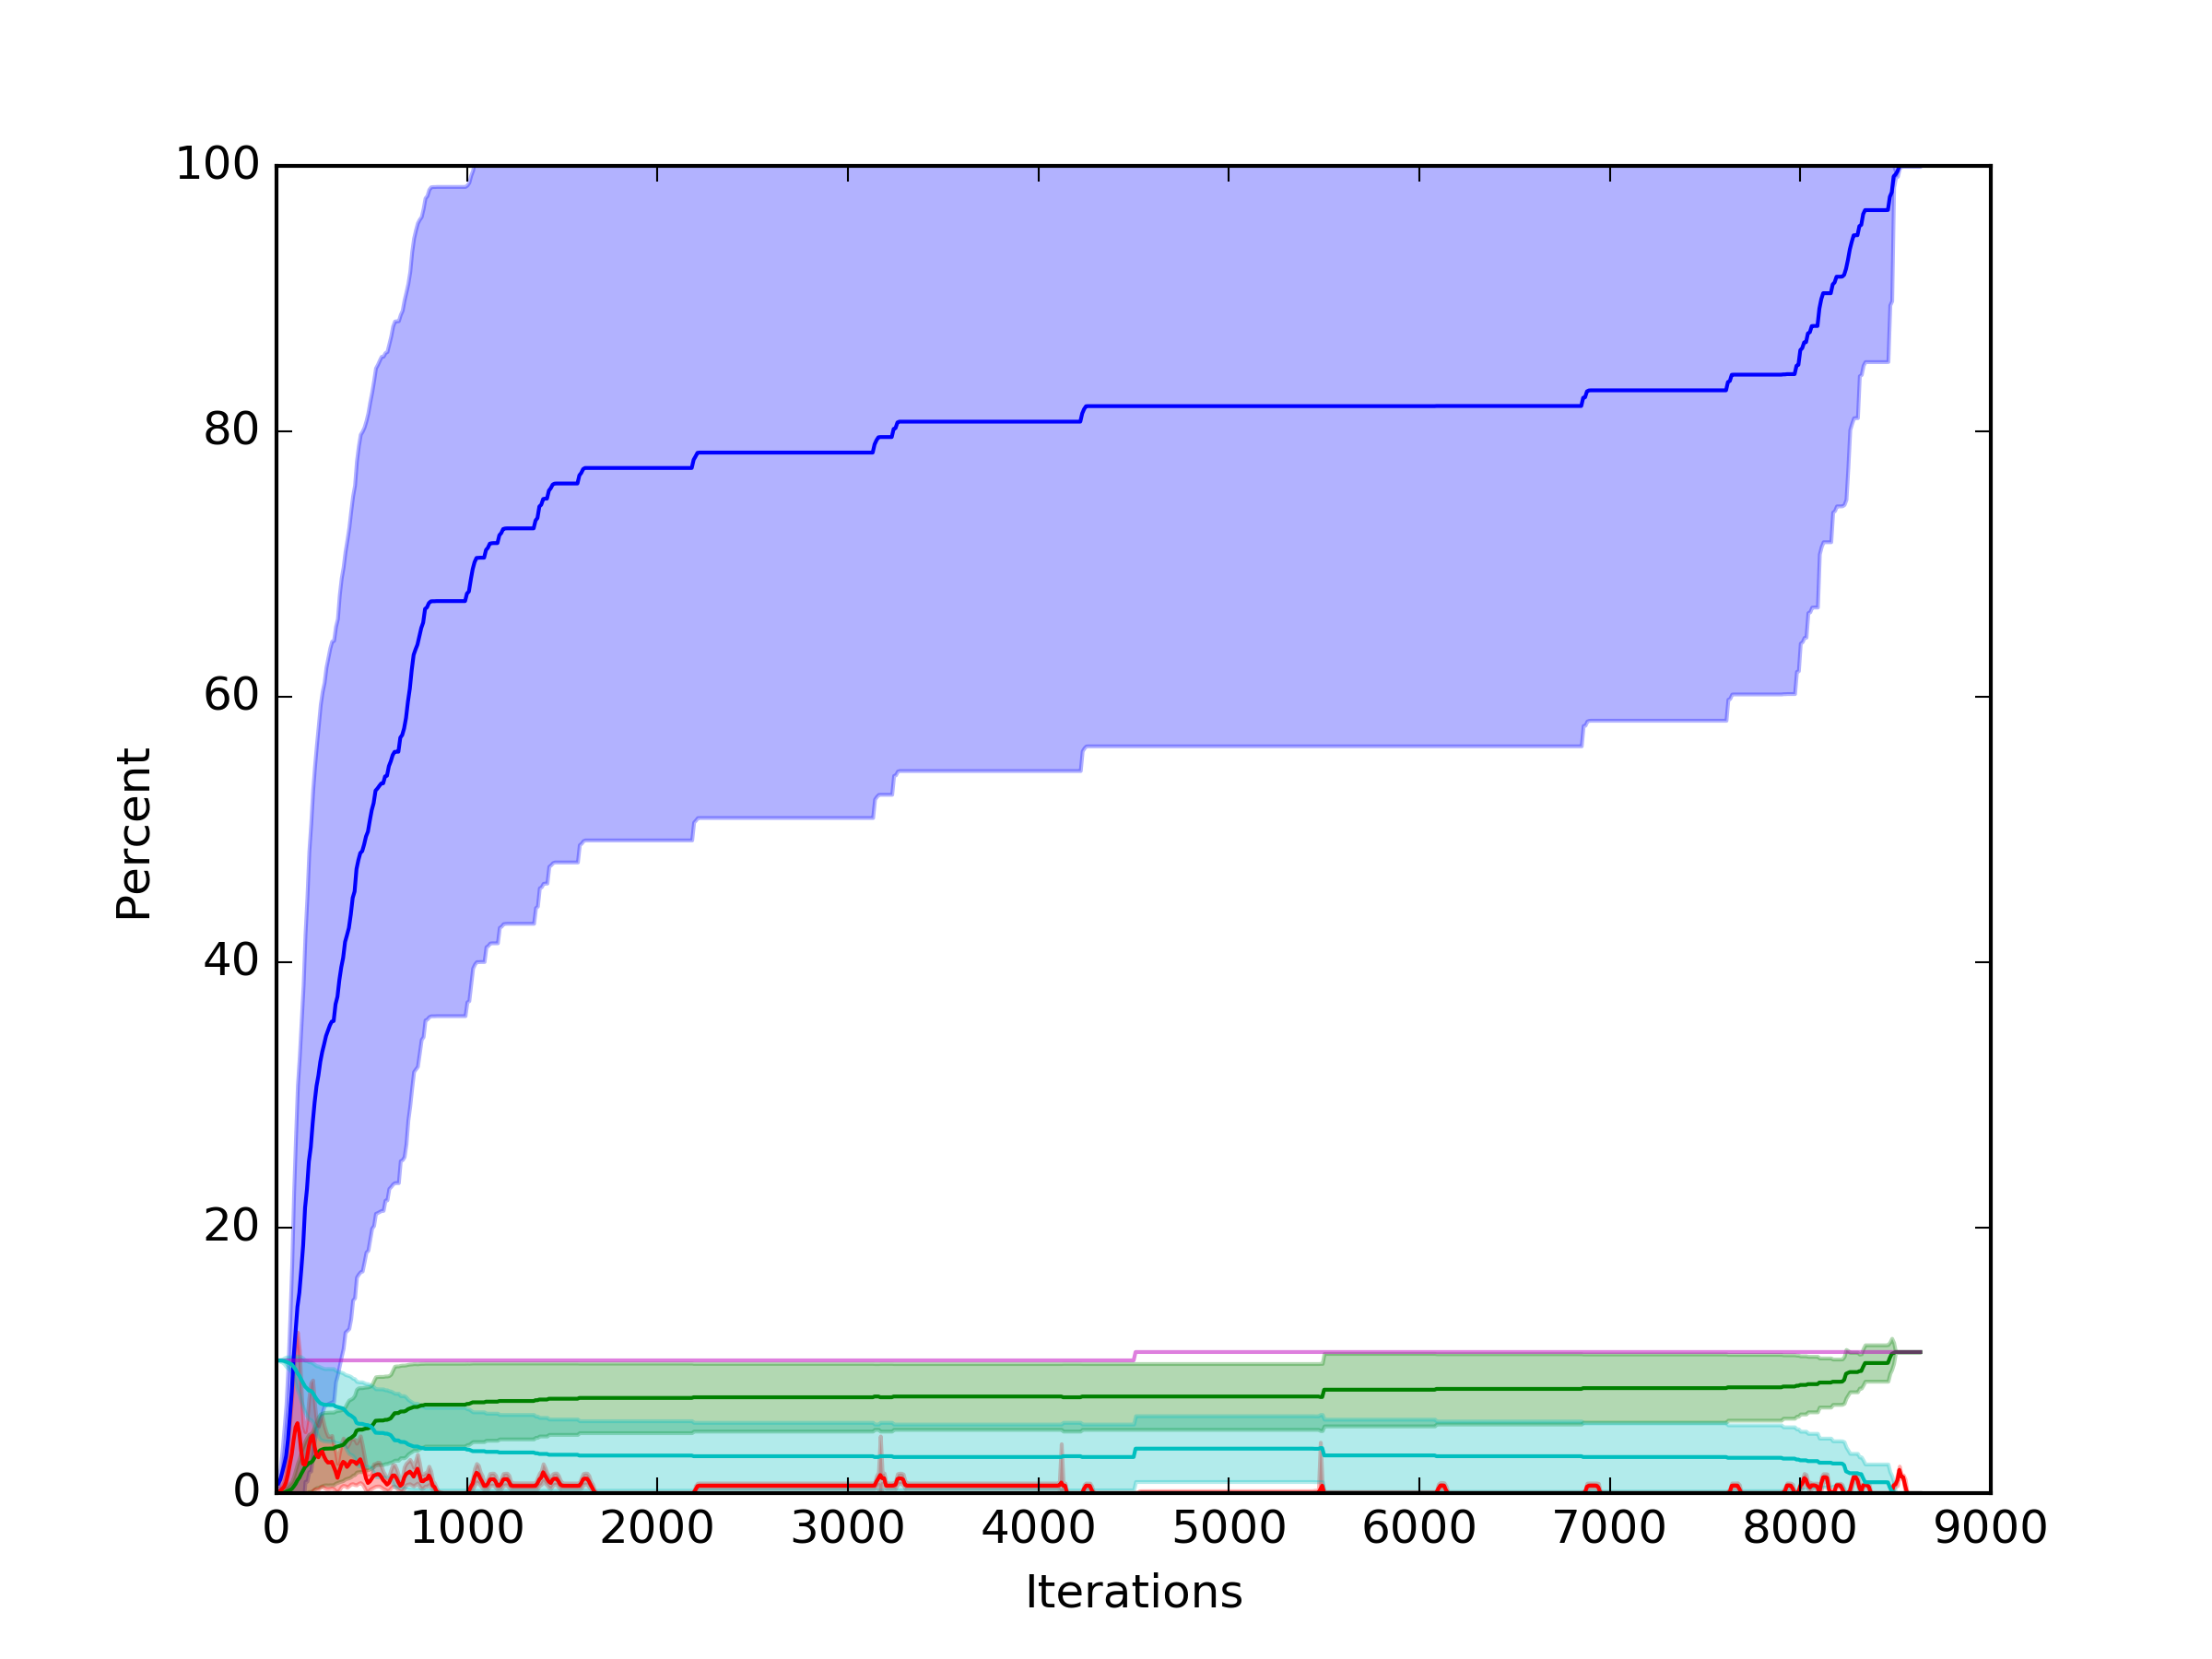
\includegraphics[width=\linewidth]{images/plots/extra_malicious/1_1000}
\caption{$m = 1000$.} \label{fig:extra1000}
\end{subfigure}

\begin{subfigure}{0.6\textwidth}
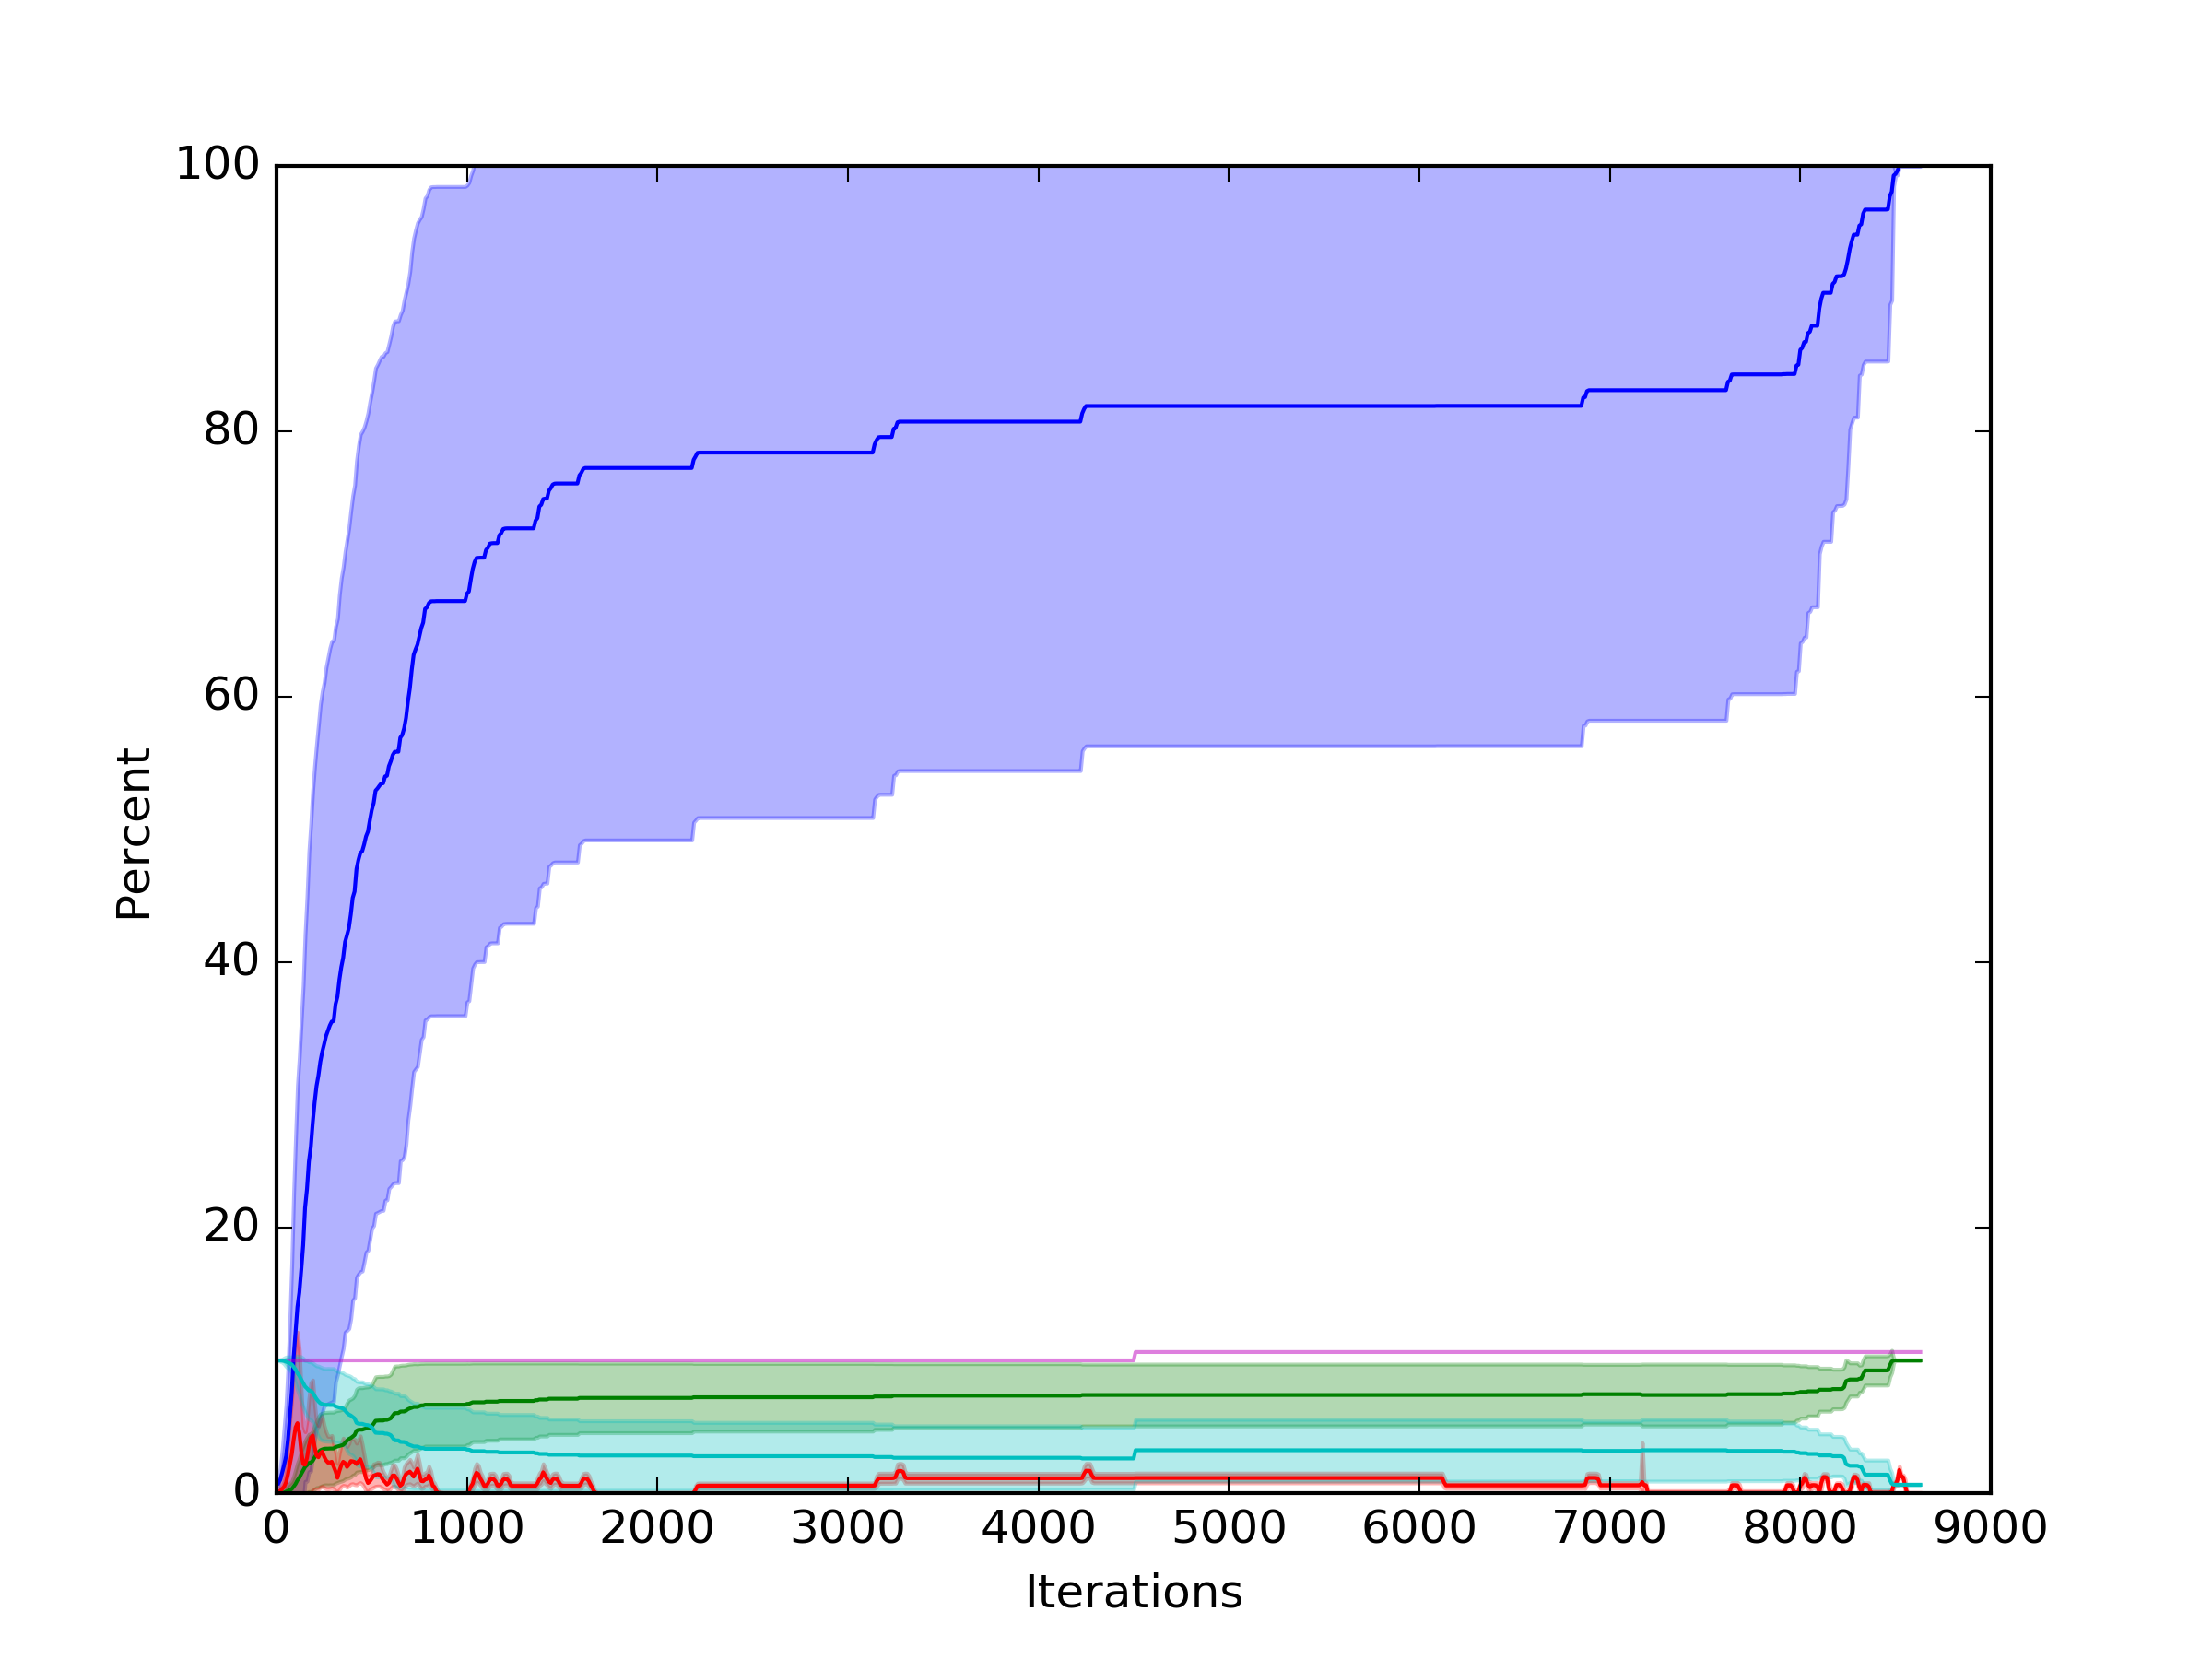
\includegraphics[width=\linewidth]{images/plots/extra_malicious/1_5000}
\caption{$m = 5000$.} \label{fig:extra5000}
\end{subfigure}

\caption{Simulation with information aging, with different maximum age values ($m=1000, 5000$).}
\label{fig:extramaliciousaging2}
\end{figure}

%\begin{figure}
%\centering
%
%\begin{subfigure}{0.4\textwidth}
%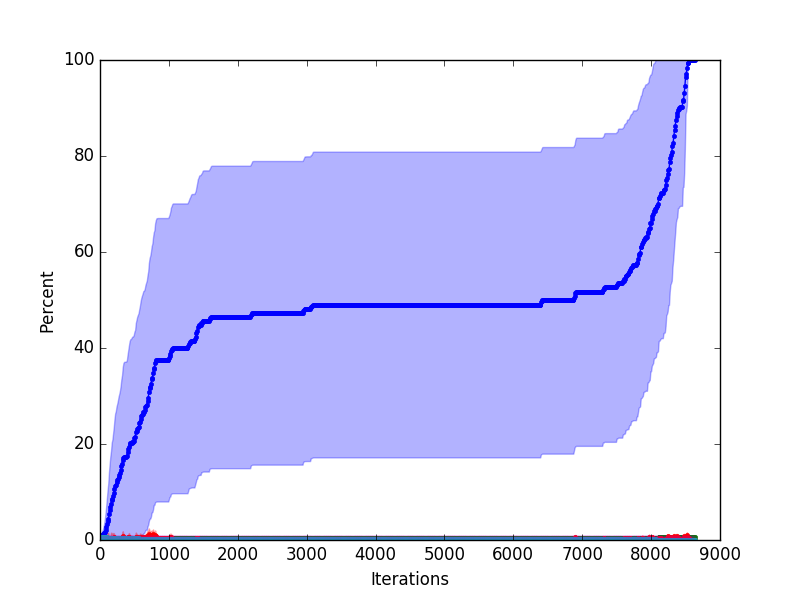
\includegraphics[width=\linewidth]{images/plots/Network_rA/10_1.png}
%\caption{1\% malicious.} \label{fig:tarjan0}
%\end{subfigure}
%
%\hspace*{1cm}
%
%\begin{subfigure}{0.4\textwidth}
%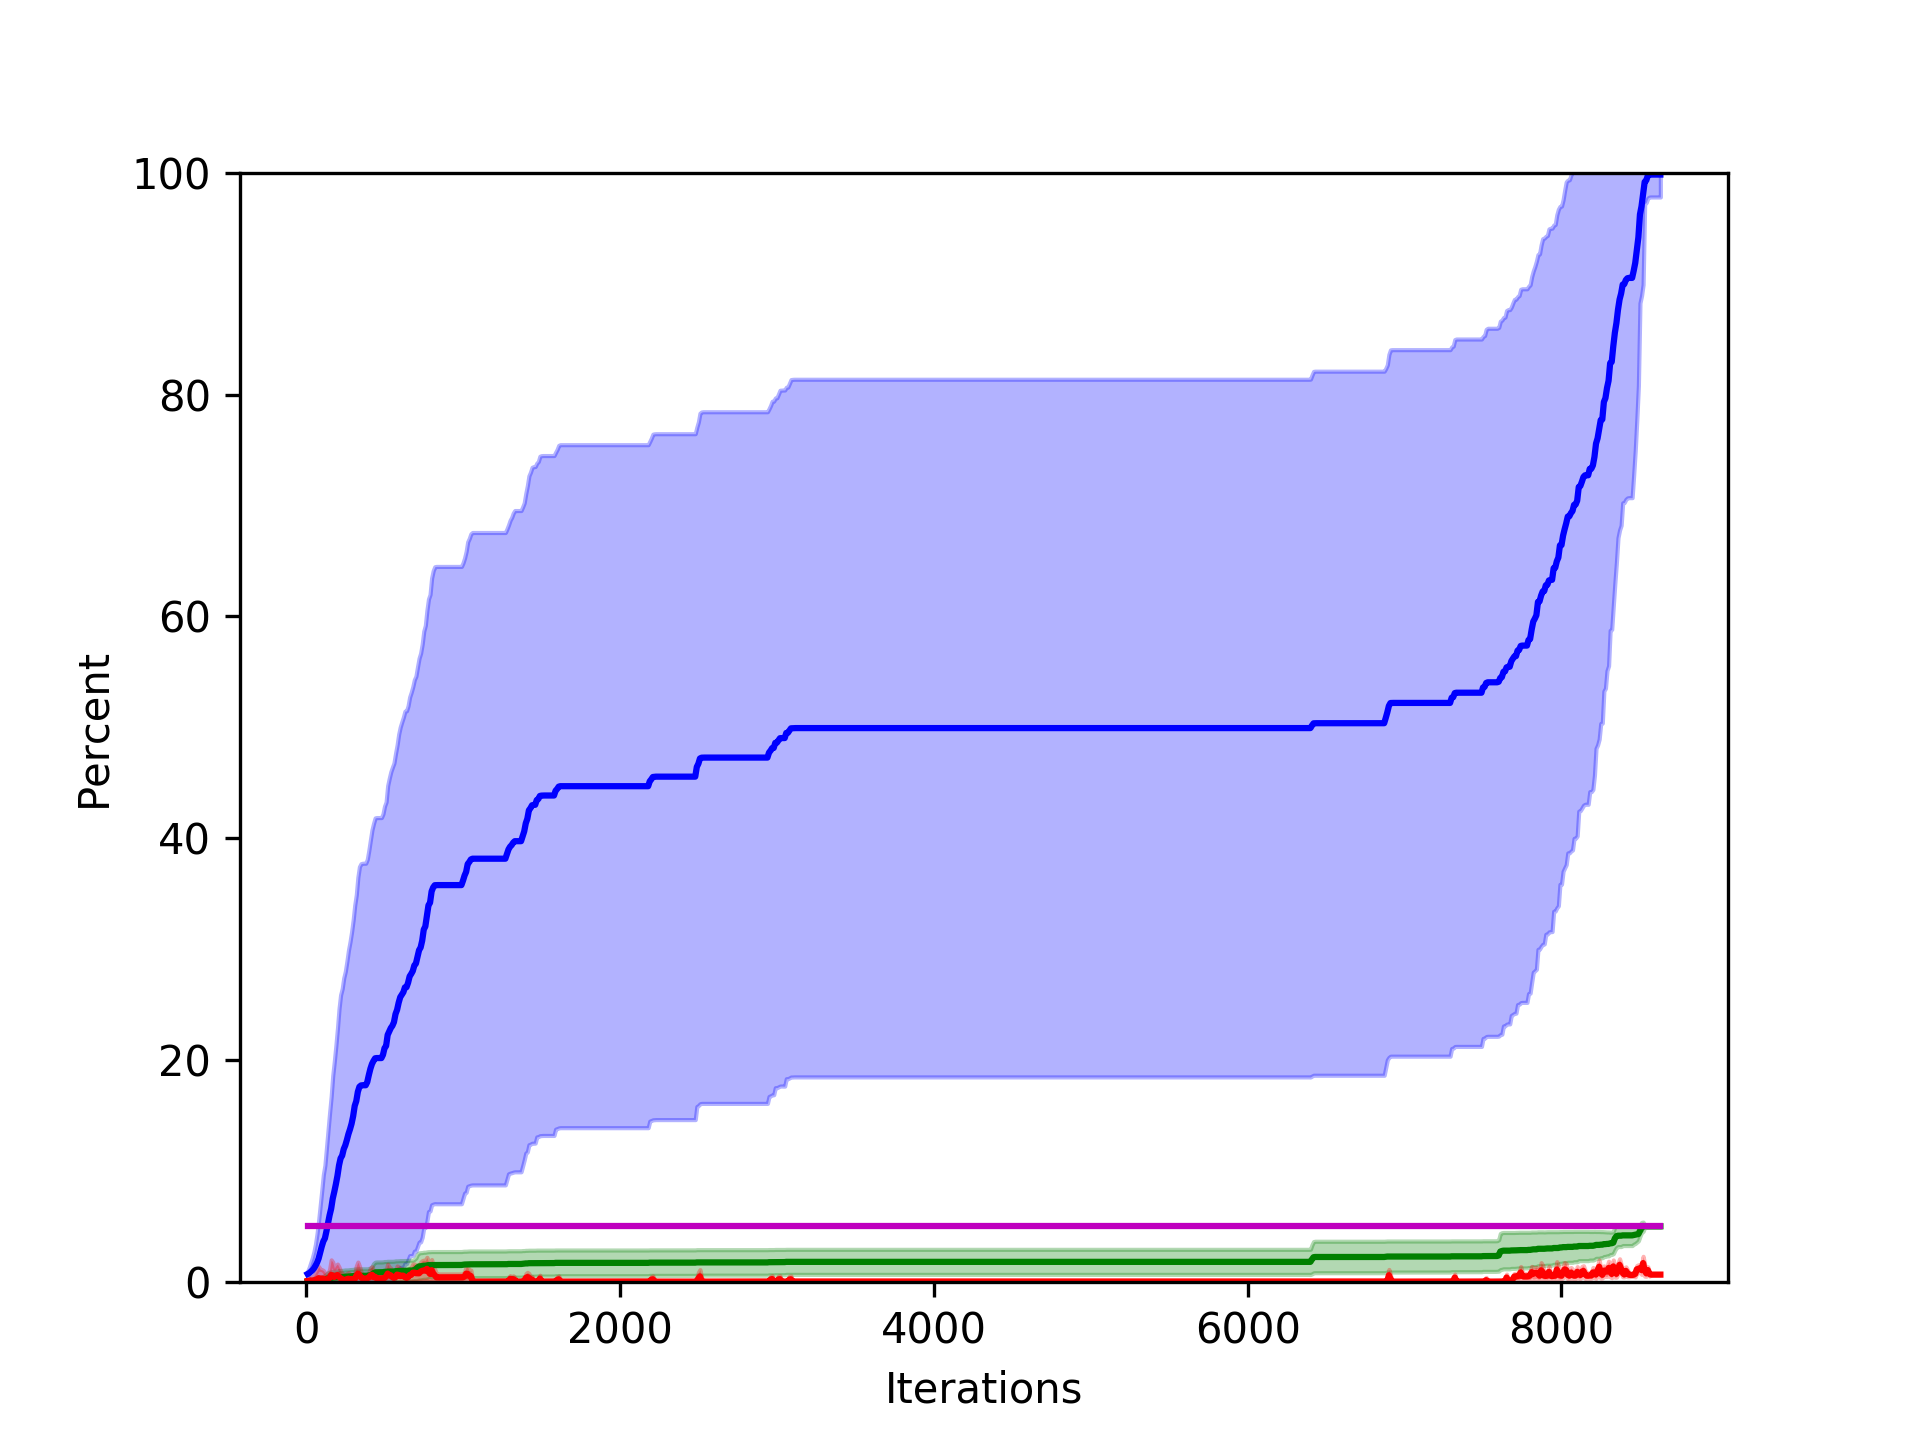
\includegraphics[width=\linewidth]{images/plots/Network_rA/10_5.png}
%\caption{5\% malicious.} \label{fig:tarjan0}
%\end{subfigure}
%
%\vspace{1cm}
%
%\begin{subfigure}{0.5\textwidth}
%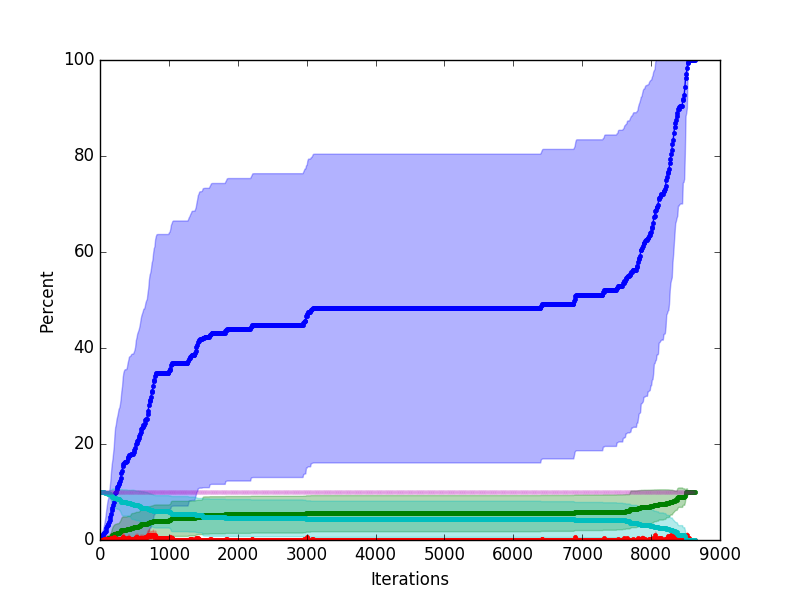
\includegraphics[width=\linewidth]{images/plots/Network_rA/10_10}
%\caption{10\% malicious.} \label{fig:tarjan0}
%\end{subfigure}
%
%\hspace*{\fill}
%
%\begin{subfigure}{0.5\textwidth}
%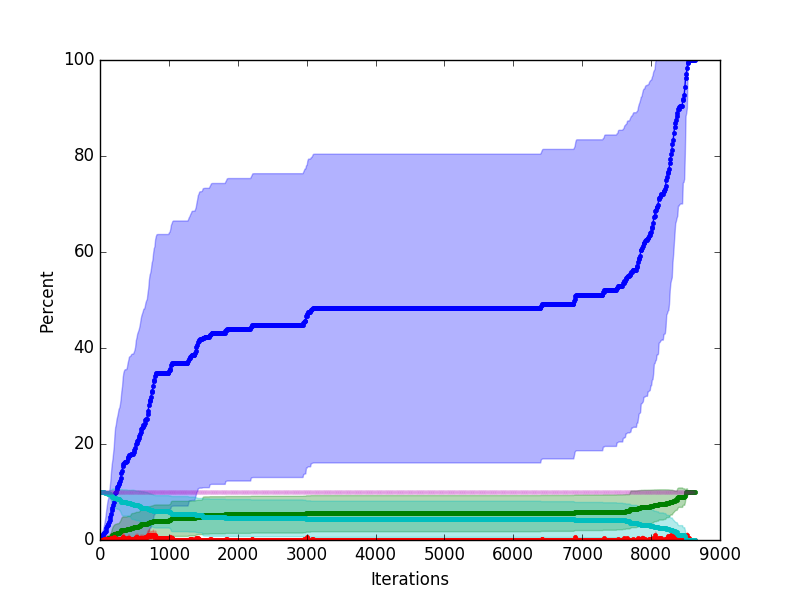
\includegraphics[width=\linewidth]{images/plots/Network_rA/10_10}
%\caption{$\rho$ = 50m.} \label{fig:tarjan0}
%\end{subfigure}
%
%\vspace{1cm}
%
%\begin{subfigure}{0.5\textwidth}
%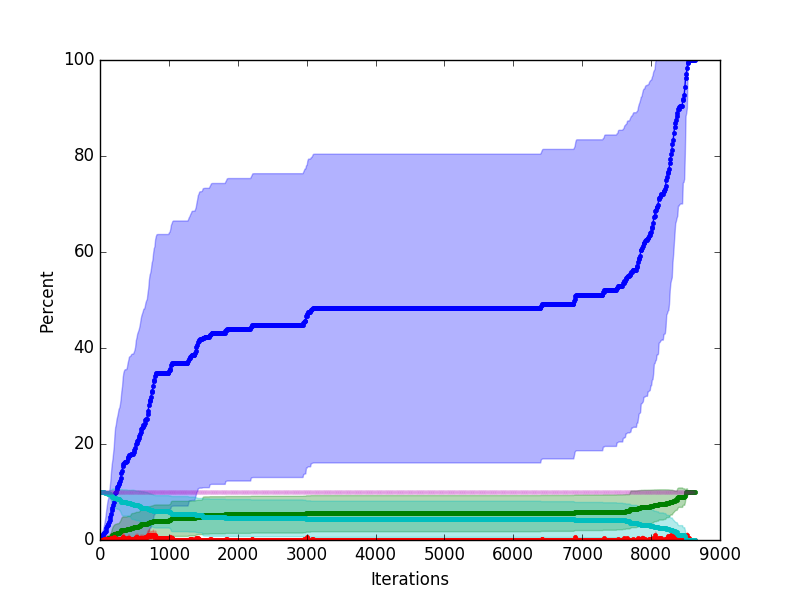
\includegraphics[width=\linewidth]{images/plots/Network_rA/10_10}
%\caption{$\rho$ = 50m.} \label{fig:tarjan0}
%\end{subfigure}
%
%\hspace*{\fill}
%
%\begin{subfigure}{0.5\textwidth}
%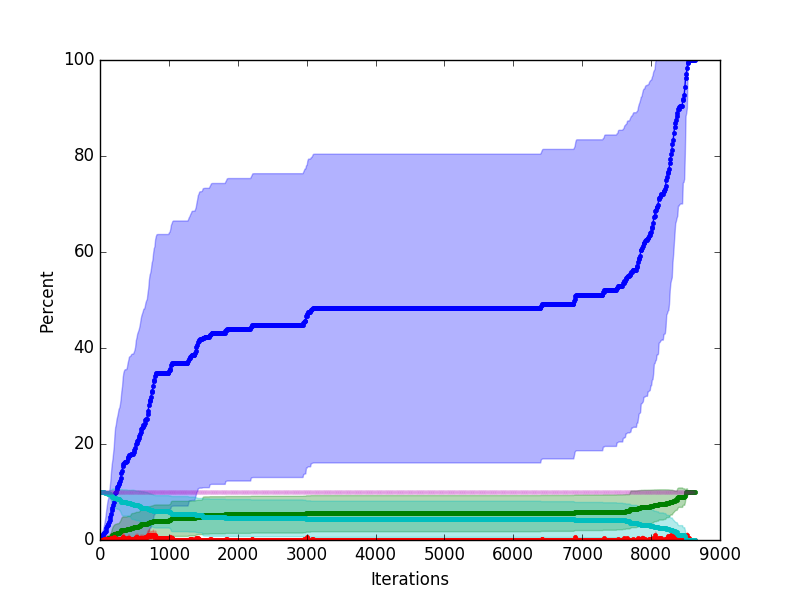
\includegraphics[width=\linewidth]{images/plots/Network_rA/10_10}
%\caption{$\rho$ = 50m.} \label{fig:tarjan0}
%\end{subfigure}
%
%\caption{Simulation with $\rho$ = 10m varying malicious.}
%\label{fig:random0}
%\end{figure}

%\begin{figure*}[!t]
%\centering
%\subfloat[]{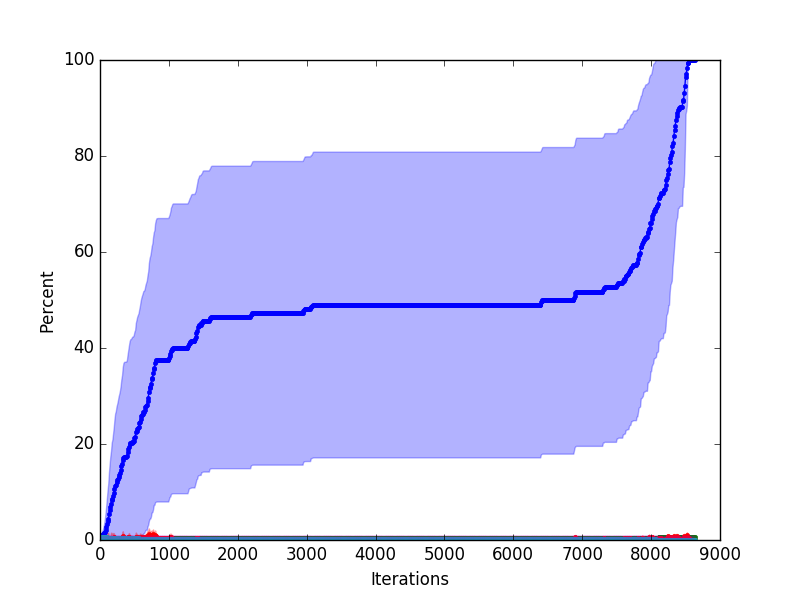
\includegraphics[width=0.329\linewidth]{images/plots/Network_rA/10_1}%
%\label{subfig:random1}}
%\hfil
%\subfloat[]{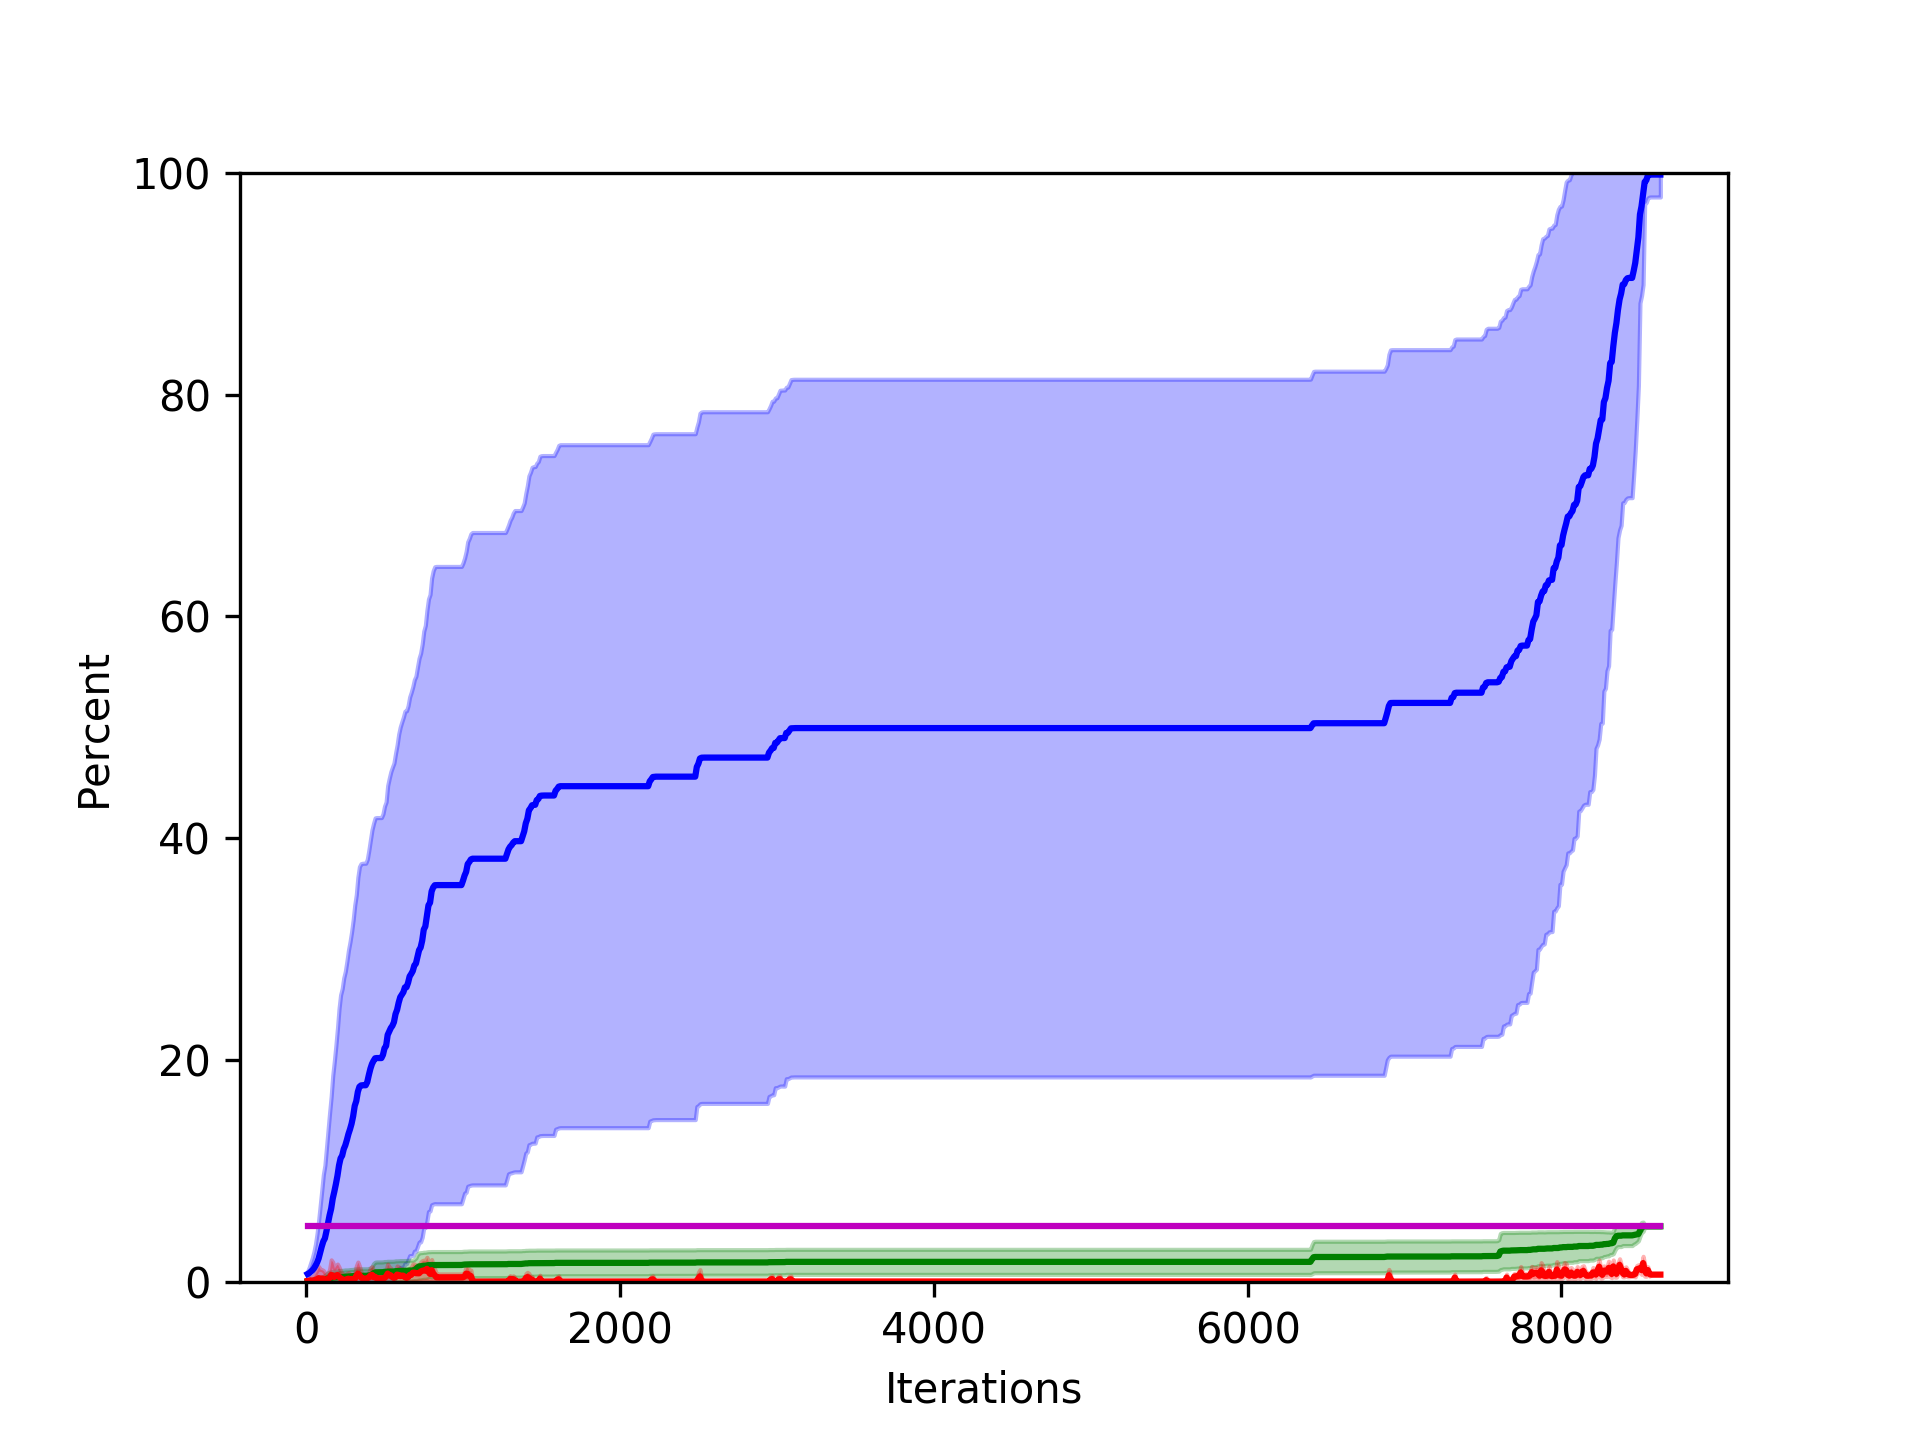
\includegraphics[width=0.329\linewidth]{images/plots/Network_rA/10_5}%
%\label{subfig:random2}}
%\hfil
%\subfloat[]{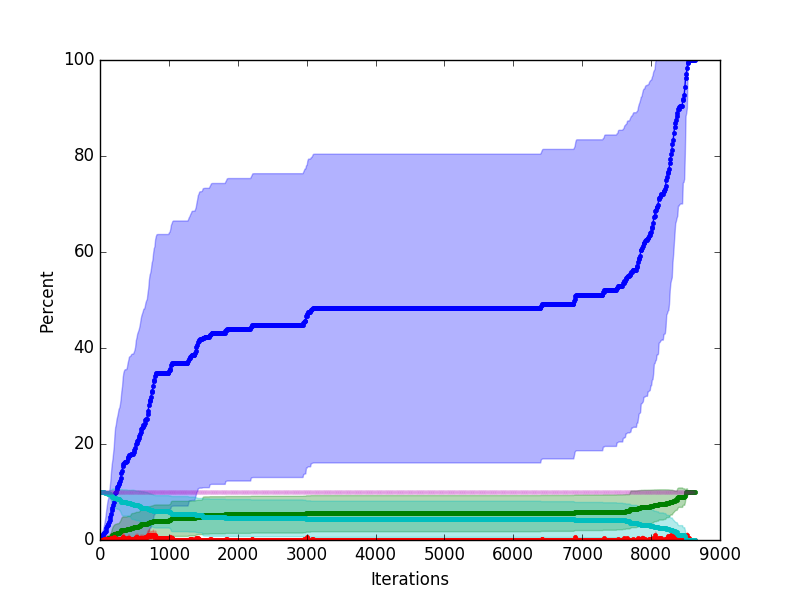
\includegraphics[width=0.329\linewidth]{images/plots/Network_rA/10_10}%
%\label{subfig:random3}}
%
%\subfloat[]{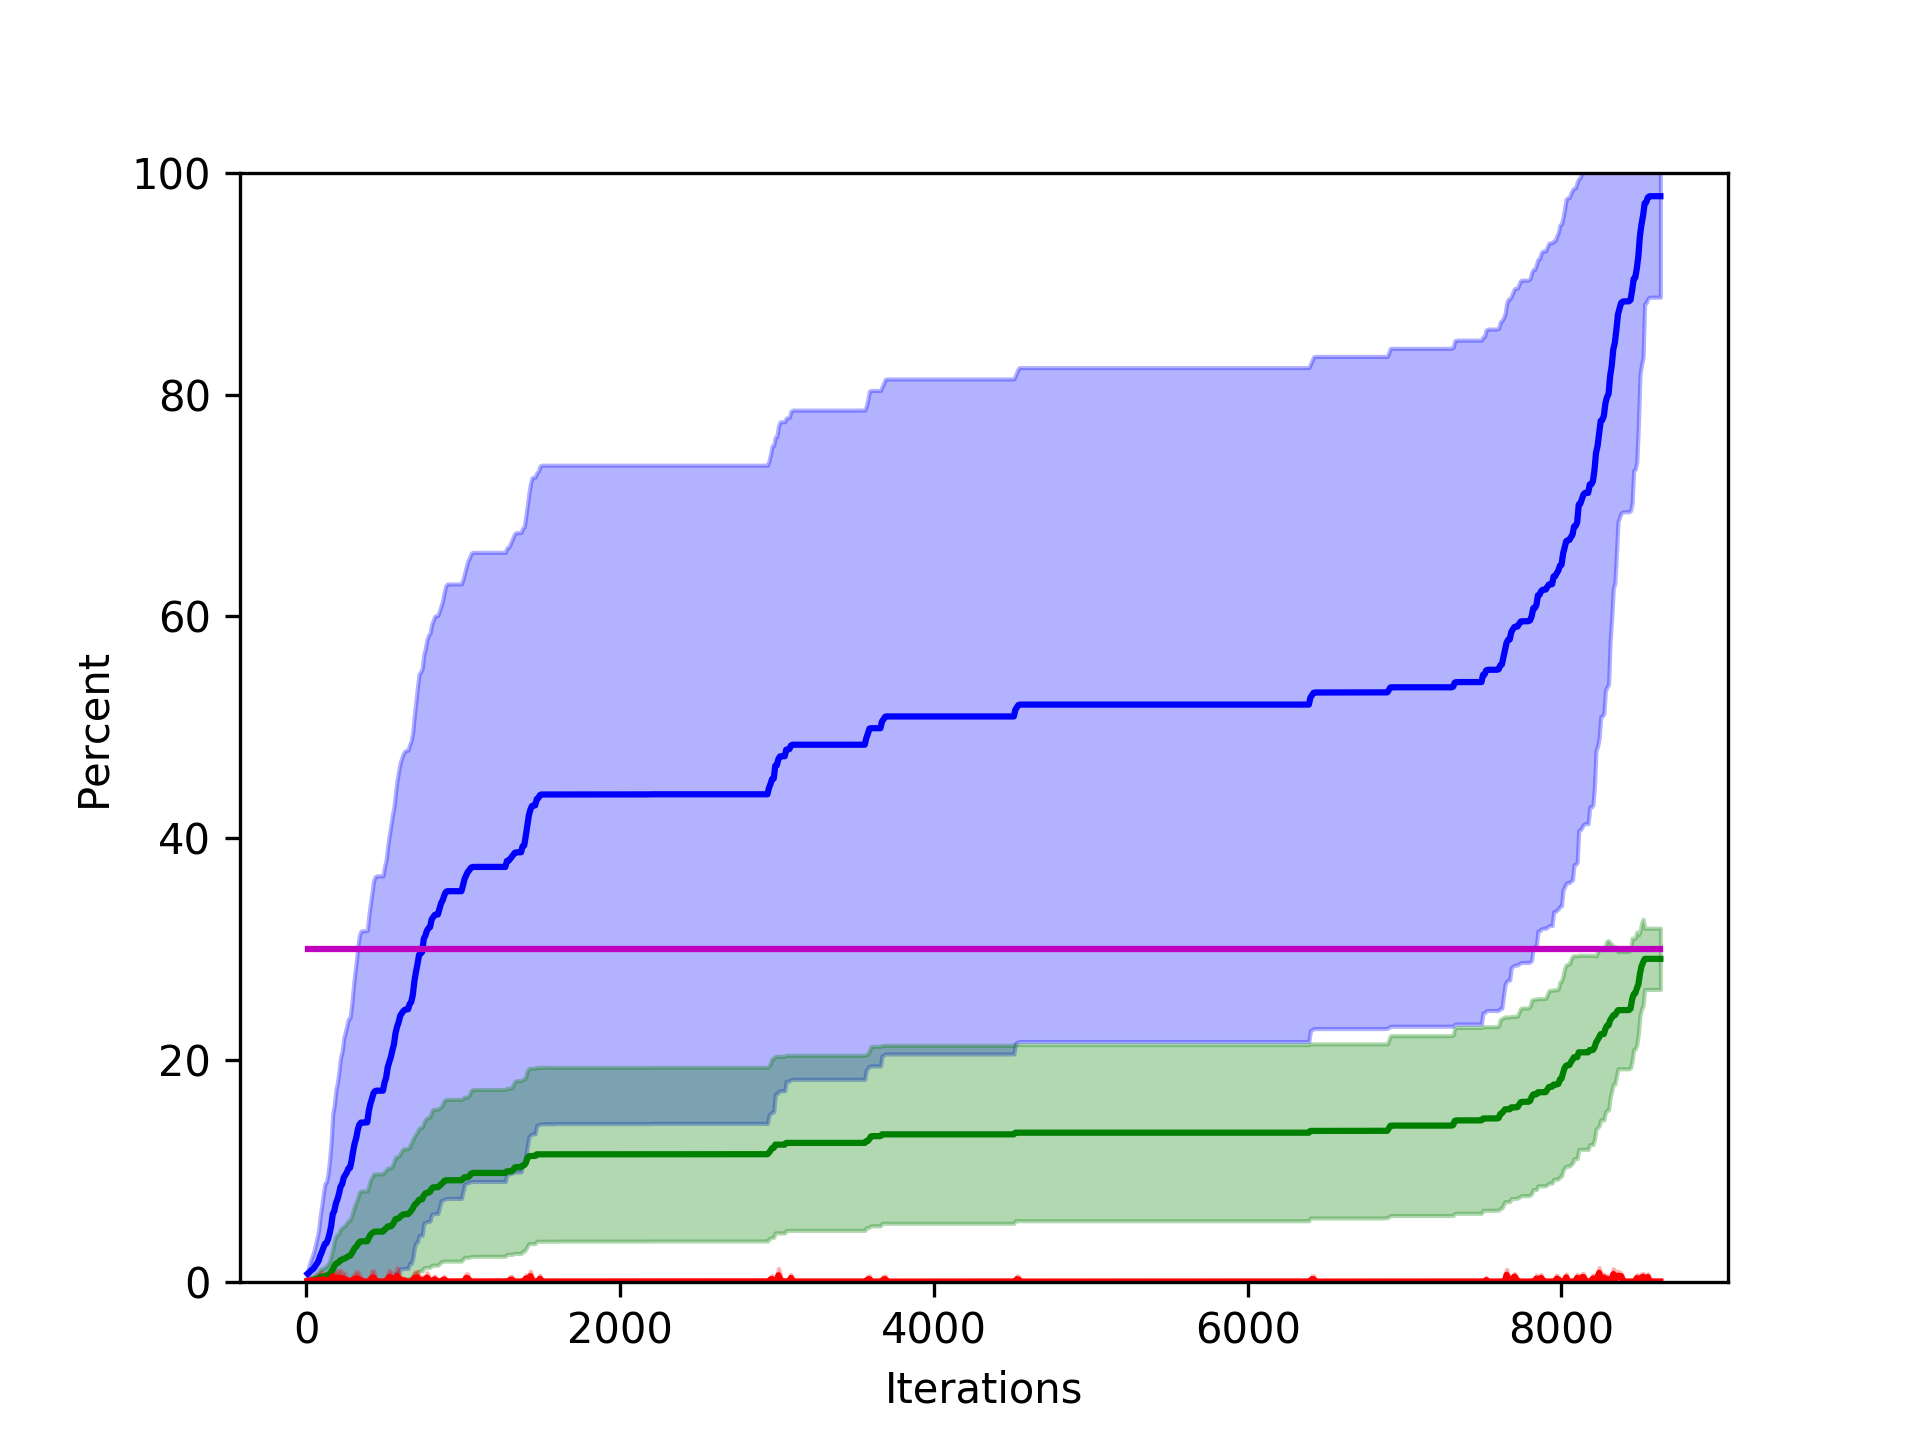
\includegraphics[width=0.329\linewidth]{images/plots/Network_rA/10_30}%
%\label{subfig:random4}}
%\hfil
%\subfloat[]{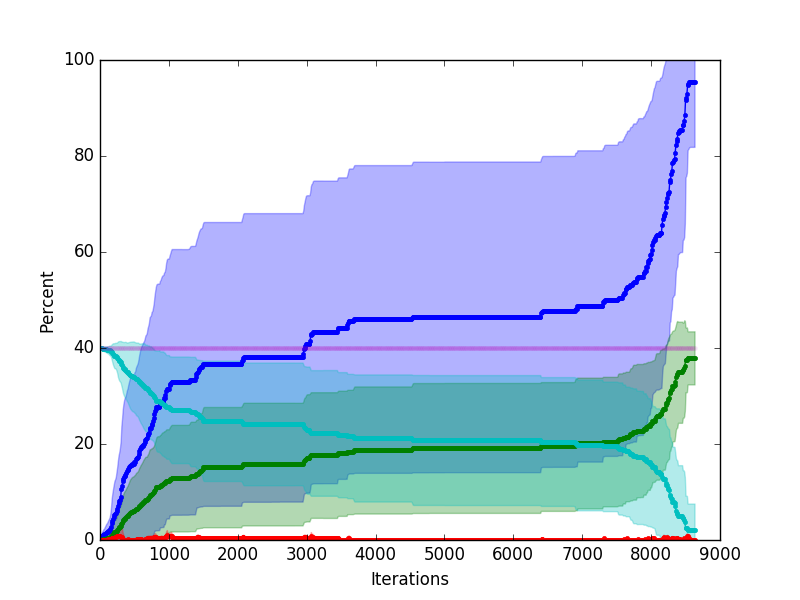
\includegraphics[width=0.329\linewidth]{images/plots/Network_rA/10_40}%
%\label{subfig:random5}}
%\hfil
%\subfloat[]{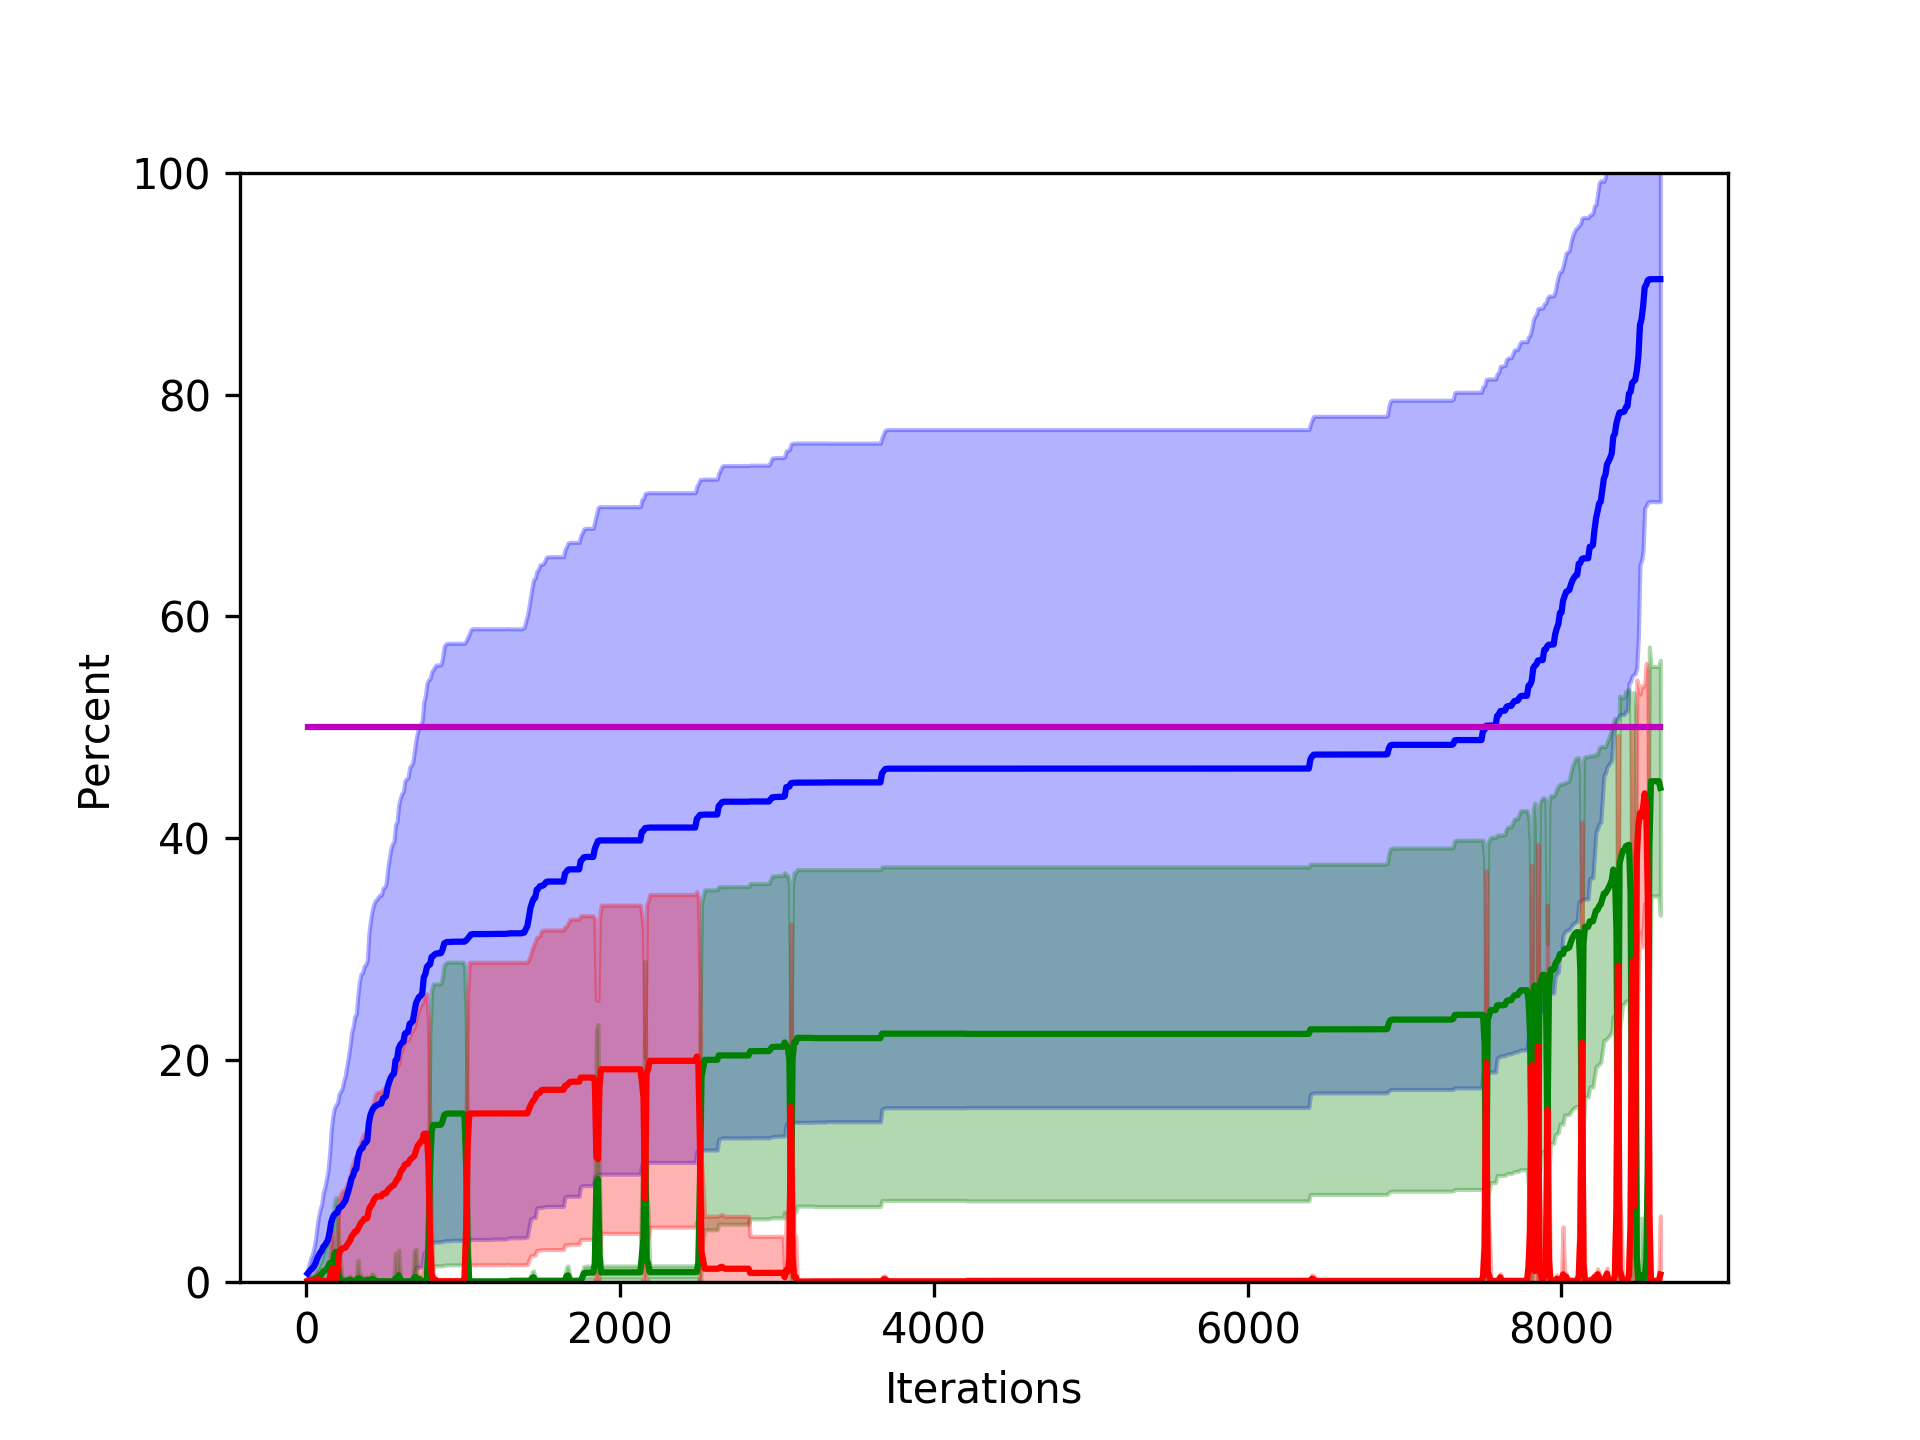
\includegraphics[width=0.329\linewidth]{images/plots/Network_rA/10_50}%
%\label{subfig:random6}}
%
%\caption{Simulation with $\rho$ = 10m and (a) 1\%, (b) 5\%, (c) 10\%, (d) 30\%, (e) 40\% or (f) 50\% malicious.}
%\label{fig:random0}
%\end{figure*}
